% THIS IS GDANSK UNIVERSITY OF TECHNLOGOGY (PG) PRESENTATION TEMPLATE
% Creator: Jan Cychnerski <jan.cychnerski@eti.pg.edu.pl>
% Copyleft 2019

% traditional screen
\documentclass{beamer}

%\usepackage{biblatex}

% Dodajemy plik bibliograficzny
%\addbibresource{lipics-v2021-sample-article.bib}
% wide screen
%\documentclass[aspectratio=169]{beamer}


%%% YOUR PACKAGES HERE %%%
\usepackage{graphicx}
\usepackage{amsmath}
\usepackage{chngcntr}
\usepackage{amsthm}
\usepackage{amsfonts}
\usepackage{amssymb}
\usepackage{indentfirst}
\usepackage{wrapfig}
\usepackage{adjustbox}
\usepackage{tikz}
\usepackage{textgreek}
\usepackage{float}
\usepackage{setspace}
\onehalfspacing
\usepackage{algorithmicx}
\usepackage{algorithm}
%\usepackage[noend, linesnumbered]{algpseudocode}
\usepackage[ruled,vlined]{algorithm2e}
\usepackage{geometry}
\usepackage{lscape}
\usepackage{appendix}
\usepackage{etoolbox}
\usepackage{tabularx}
\usepackage{array}
\usepackage{caption}
\usepackage{boxedminipage}
\usepackage[most]{tcolorbox}
\tcbuselibrary{breakable}
\usetikzlibrary{shadows}
\usepackage{hyperref}

\usepackage{etoolbox} % Pakiet pomocniczy

\usepackage{lipsum}


\usepackage{graphicx}
\usepackage{amsmath}
\usepackage{chngcntr}
\usepackage{amsthm}
\usepackage{amsfonts}
\usepackage{amssymb}
\usepackage{indentfirst}
\usepackage{wrapfig}
\usepackage{adjustbox}
\usepackage{tikz}
\usepackage{textgreek}
\usepackage{float}
\usepackage{setspace}
\onehalfspacing
\usepackage[hidelinks]{hyperref}
\usepackage[ruled,vlined]{algorithm2e}
\SetArgSty{textnormal} 
\usepackage{geometry}
\usepackage{lscape}
\usepackage{appendix}
\usepackage{etoolbox}
\usepackage{tabularx}
\usepackage{array}
\usepackage{caption}
\usepackage{boxedminipage}
\usepackage[most]{tcolorbox}
\tcbuselibrary{breakable}
\usetikzlibrary{shadows}
\usetikzlibrary{decorations.pathreplacing,calligraphy,backgrounds}
\usetikzlibrary{shapes.geometric}
\usetikzlibrary{arrows.meta}
\usetikzlibrary{3d, calc}
\usepackage{tikz-3dplot}



% polish language
%\usepackage[polish]{babel}
%\usepackage{polski}

\newcommand{\br}[1]{\left( #1 \right)}
\newcommand{\brc}[1]{\left\{ #1 \right\}}
\newcommand{\spr}[1]{\left| #1 \right|}
\newcommand{\fl}[1]{\left\lfloor #1 \right\rfloor}
\newcommand{\cl}[1]{\left\lceil #1 \right\rceil}
\newcommand{\angl}[1]{\langle #1 \rangle}
\newcommand{\e}[1]{\exp\left\{ #1 \right\}}
\newcommand{\ecc}{\operatorname{ecc}}
\newcommand{\rad}{\operatorname{rad}}
\newcommand{\diam}{\operatorname{diam}}
\newcommand{\Rim}{\operatorname{Rim}}
\newcommand{\rim}{\operatorname{rim}}
\newcommand{\Anc}{\operatorname{Anc}}
\newcommand{\NPcomplete}{\textnormal{$\mathcal{NP}$-Complete}}
\newcommand{\NPhard}{\textnormal{$\mathcal{NP}$-Hard}}
\newcommand{\polyAPXcomplete}{\textnormal{Poly-$\mathcal{APX}$-Complete}}
\newcommand{\Cent}{\texttt{Cent}}
\newcommand{\APP}{\texttt{APP}}
\newcommand{\OPT}{\texttt{OPT}}
\newcommand{\COST}{\texttt{COST}}
\newcommand{\LB}{\mathcal{LB}}
\newcommand{\HB}{\mathcal{HB}}
\newcommand{\THB}{\mathcal{THB}}
\newcommand{\THH}{\texttt{TH}}
\newcommand{\argmin}{\operatorname*{arg\,min}}
\newcommand{\argmax}{\operatorname*{arg\,max}}


\SetKwFunction{FMergeDTs}{MergeDTs}
\SetKwFunction{FQPTAS}{QPTAS}
\SetKwFunction{FRankingBasedDT}{RankingBasedDT}
\SetKwFunction{FDPTimelinesCosts}{DPTimelinesCosts}
\SetKwFunction{FApproxDT}{ApproxDT}


\makeatletter

%%% IMPORT PG PRESENTATION STYLE %%%
% THIS IS GDANSK UNIVERSITY OF TECHNLOGOGY (PG) PRESENTATION TEMPLATE
% Creator: Jan Cychnerski <jan.cychnerski@eti.pg.edu.pl>
% Copyleft 2019


% PG THEME OPTIONS

\usetheme{Boadilla}
\usecolortheme{default}
\usefonttheme{professionalfonts}

% colors

\definecolor{PGBlue}{RGB}{0,56,101}
\definecolor{PGRed}{RGB}{193,10,39}
\definecolor{PGSilver}{RGB}{200,200,200}
\definecolor{PGBlack}{RGB}{0,0,0}

% PGBlue
\setbeamercolor{frametitle}{fg=PGBlue}
\setbeamercolor{normal text}{fg=PGBlue}
\setbeamercolor{structure}{fg=PGBlue}
\setbeamercolor{item}{fg=PGBlue}

% PGRed
\setbeamercolor{alerted text}{fg=PGRed}
\setbeamercolor{item projected}{fg=PGRed}

% white
\setbeamercolor{title}{fg=white}
\setbeamercolor{titlelike}{fg=white}
\setbeamercolor{subtitle}{fg=white}

% enumerate and itemize styles

\setbeamertemplate{itemize item}{\bfseries\color{PGRed}\raise1pt\hbox{\donotcoloroutermaths$\bullet$}}
\setbeamertemplate{itemize subitem}{\color{PGRed}\raise0.5pt\hbox{--}}
\setbeamertemplate{itemize subsubitem}{\color{PGRed}\tiny\raise1.5pt\hbox{\donotcoloroutermaths$\bullet$}}

\setbeamertemplate{enumerate item}{\bfseries\color{PGRed}\insertenumlabel.}
\setbeamertemplate{enumerate subitem}{\color{PGRed}\insertsubenumlabel.}
\setbeamertemplate{enumerate subsubitem}{\color{PGRed}\insertsubsubenumlabel.}
\setbeamertemplate{enumerate mini template}{\insertenumlabel}


% disable navigation

\beamertemplatenavigationsymbolsempty

% additional commands

\newcommand*{\vcenteredhbox}[1]{\begingroup
\setbox0=\hbox{#1}\parbox{\wd0}{\box0}\endgroup}

\graphicspath{{pgbeamer/}}


\usepackage{iflang}
\IfLanguageName{polish}{
\newcommand{\pglogobig}{pg-logo-big-pl}
\newcommand{\pglogosmall}{pg-logo-small-pl}
}{
\newcommand{\pglogobig}{pg-logo-big-en}
\newcommand{\pglogosmall}{pg-logo-small-en}
}


% FRAME TITLE LOGO
\addtobeamertemplate{frametitle}{\vcenteredhbox{\includegraphics[height=8mm]{\pglogosmall}}\bfseries}{}


\newcommand{\pgtitleframe}{{
% PG TITLE PAGE

\setbeamercolor{background canvas}{bg=PGBlue}
\setbeamercolor{title}{fg=white}
\setbeamercolor*{date}{fg=white}
\setbeamercolor*{author}{fg=white}

\setbeamertemplate{footline}{}

\begin{frame}[noframenumbering]
\centering
\vspace{1cm}
\includegraphics[height=3cm]{\pglogobig}
\vspace{5mm}
\maketitle
\end{frame}
}}

\newcommand{\pglastframe}{{
% PG LAST PAGE

\setbeamercolor{background canvas}{bg=PGBlue}
\setbeamercolor{title}{fg=white}
\setbeamercolor*{date}{fg=white}
\setbeamercolor*{author}{fg=white}

\setbeamertemplate{footline}{}

\begin{frame}[noframenumbering]
\centering
\vspace{1cm}
\includegraphics[height=5cm]{\pglogobig}
\end{frame}
}}




%%% YOUR OPTIONS HERE %%%

\title[PG Presentation]{Experimental analysis of binary search models in graphs}
\subtitle{\textbf{Supervised by:} prof. dr. hab. inż. Dariusz Dereniowski}
\author{Michał Szyfelbein}

\date{\today}

\setbeamercovered{transparent}
%%% DOCUMENT BEGINS HERE %%%

\begin{document}


\usetikzlibrary {graphs,graphdrawing} 
\usegdlibrary {trees, layered, force}

%%% PG TITLE PAGE %%%
\pgtitleframe

%%% YOUR PRESENTATION HERE %%%


\begin{frame}{Basic information}
	\textbf{The aim:} Experimental analysis of selected generalized binary search problems. The aim of the analysis is to verify the hypotheses regarding the effectiveness of search algorithms. 
    
    \textbf{Schedule:}
    \begin{itemize}
    \pause
    \item 2024.01 -- 2024.06: Researching and selection of the query model.
    \item 2024.06 -- 2025.05: Development and formal analysis of the proposed algorithms.
    \item 2025.06 -- 2025.10: Selection of models and algorithms for comparison, implementation, thesis writing.
    \item 2025.11 -- 2025.12: execution of experiments, analysis and interpretation of the results, finalization of the thesis.

\end{itemize}
\end{frame}

\begin{frame}{State of the work}
    \begin{itemize}
        \item Implementation, about 60\% complete:
        \begin{itemize}
        \item Language: \textbf{python},
        \item Libraries: \textbf{networkx},
        \item Environment: \textbf{PyCharm},
        \item Versioning: \textbf{git} + \textbf{github}, \hyperlink{https://github.com/MSzyfel/Binary-Search}{https://github.com/MSzyfel/Binary-Search}.
        \end{itemize} 
        \pause
        \item Thesis, about 80\% complete:
        \begin{itemize}
            \item Language: \textbf{LaTeX},
            \item Environment: \textbf{Visual Studio Code},
            \item Versioning: \textbf{git} + \textbf{github}, \hyperlink{https://github.com/MSzyfel/Papers}{https://github.com/MSzyfel/Papers}.
        \end{itemize} 
        \pause
        \item What is left: 
        \begin{itemize}
            \item Experiments,
            \item Advanced data generation,
            \item Optimization,
            \item Bug fixing,
            \item Data visualization.
        \end{itemize} 
    \end{itemize}
\end{frame}
\begin{frame}{Binary Search}
    
\begin{figure}[ht]
\centering
\begin{tikzpicture}[every node/.style={font=\small}, scale=0.75]

% --- Array values (10 elements) ---
\def\A{{1, 2, 4, 5, 7, 10, 15, 16, 18, 21, 22, 25, 31, 32}}
\def\MID{6} % Index of median (0-based): value = 23
% Draw array elements and indices
\foreach \i in {0,...,13} {
    \pgfmathsetmacro{\val}{\A[\i]}
    \draw[thick] (\i, 0) rectangle ++(1,1);
    \node at (\i+0.5, 0.5) {\val};
}

% Underline LEFT subarray (0..3)
\draw[thick] (0.1, -0.2) -- (6.0-0.1, -0.2);
% Label
\node[below=6pt] at (3, -0.2) {lesser than median};

% Underline RIGHT subarray (5..9)
\draw[thick] (7+0.1, -0.2) -- (13+1-0.1, -0.2);
% Label
\node[below=6pt] at (10.5, -0.2) {greater than median};

% Arrow for mid
\draw[<-, thick] (\MID+0.5, 1.2) -- +(0, 0.5) node[above] {median};

\end{tikzpicture}
\caption[Binary search]{Example of a sorted array containing 14 elements. }
\label{fig:binary-search-subarrays}
\end{figure}

\end{frame}


\begin{frame}{Generalized binary search}
        \begin{definition} A \textbf{searcher} is required to find a hidden \textbf{target} vertex $x$ in a graph $G$. To do so, they iteratively perform \textbf{queries} to an \textbf{oracle}, each about a chosen vertex $v$. After each such call, the oracle responds whether the target was found and if not, the searcher receives as a reply the connected component of $G-v$ containing the target.
        \end{definition}
	\pause

	A further generalization is to associate with each vertex a \textbf{cost} function $c:V\br{G}\to \mathbb{R}_{\geq 0}$ representing the time required to query a given vertex. 
    
\end{frame}
\begin{frame}{Example}
    \begin{figure}[htbp]
    \centering
    \begin{minipage}{0.3\textwidth}
        \centering
        \tikz [tree layout, grow=-65,
               sibling distance=11mm, level distance=13mm, scale = 0.6, thick]
          \graph {
    ""[as=$a$] -- {
        ""[as=$b$, draw=red, thick, circle] -- ""[as=$c$] -- {
            ""[as=$d$] -- ""[as=$e$],
            ""[as=$f$] -- { ""[as=$g$], ""[as=$h$], ""[as=$i$] }
        },
        ""[as=$j$] -- ""[as=$k$] -- { ""[as=$l$], ""[as=$m$] }
    }
};
    \caption{Query to $b$}
    \end{minipage}
    \pause
    \begin{minipage}{0.3\textwidth}
        \centering
        \tikz [tree layout, grow=-65,
               sibling distance=11mm, level distance=13mm, scale = 0.6, thick]
          \graph {
        ""[as=$c$] -- {
            ""[as=$d$] -- ""[as=$e$],
            ""[as=$f$, draw=red, thick, circle] -- { ""[as=$g$], ""[as=$h$], ""[as=$i$]
        }
    }
};
    \caption{Query to $f$}
    \end{minipage}
    
    \pause
    \begin{minipage}{0.3\textwidth}
        \centering
        \tikz [tree layout, grow=-65,
               sibling distance=11mm, level distance=13mm, scale = 0.6, thick]
          \graph {
        ""[as=$c$] -- {
            ""[as=$d$, draw=red, thick, circle] -- ""[as=$e$]
        }
};
    \caption{Query to $d$}
    \end{minipage}
    \pause
    \begin{minipage}{0.3\textwidth}
        \centering
        \tikz [tree layout, grow=-65,
               sibling distance=11mm, level distance=13mm, scale = 0.6, thick]
          \graph {
        ""[as=$c$, draw=red, thick, circle]
};
    \caption{Query to $c$}
    \end{minipage}
\end{figure}
\end{frame}


\begin{frame}{Classes of graphs considered}
	\textbf{There are three main classes of graphs to be considered}:
	\begin{itemize}
	\item \textbf{Paths} - equivalent to searching in a sorted array. 
    \pause
	\item \textbf{Trees} -  The most extensively studied model. \textbf{Our choice}.
    \pause
    \item \textbf{General graphs} - Computationally hardest.
	\end{itemize}
\end{frame}

\begin{frame}{Decision trees}
        \begin{definition}
        A decision tree:
        \begin{itemize}
            \item $D=(V\br{D}, E\br{D})$, $V\br{D}=V\br{T}$ are vertices and $E\br{D}$ are edges of $D$.
            \pause
            \item $Q_D\br{T,x}$ - sequence of queries performed in order to find $x$.
            \pause
            \item Cost of $D$ in $\br{T,c}$:
            $$
\COST_D\br{T, c} = \max_{x\in V\br{T}} \brc{\sum_{q\in Q_{D}\br{T,x}}c\br{q}}.
$$
            \pause
        \item $\OPT(T, c) = \min_{D} \brc{\COST_D\br{T, w}}$.
        \end{itemize}
        \end{definition}
\end{frame}

\begin{frame}{Example of decision tree}
    
\begin{figure}[htbp]
    \centering
    \begin{minipage}{0.34\textwidth}
        \centering
        \tikz [tree layout, grow=-65,
               sibling distance=11mm, level distance=13mm,]
          \graph {
    ""[as=$a$] -- {
        ""[as=$b$] -- ""[as=$c$] -- {
            ""[as=$d$] -- ""[as=$e$],
            ""[as=$f$] -- { ""[as=$g$], ""[as=$h$], ""[as=$i$] }
        },
        ""[as=$j$] -- ""[as=$k$] -- { ""[as=$l$], ""[as=$m$] }
    }
};
    \caption[Sample tree]{}
    \label{fig:tree}
    \end{minipage}
    \begin{minipage}{0.32\textwidth}
        \centering
        \tikz [tree layout, grow=-90,
               sibling distance=12mm, level distance=14mm,]
          \graph {
            ""[as=$c$] -> { ""[as=$j$] -> { ""[as=$a$] -> ""[as=$b$],  ""[as=$l$] -> {""[as=$k$] -> ""[as=$m$]}}, ""[as=$h$] -> {""[as=$f$] -> {""[as=$g$], ""[as=$i$]}},  ""[as=$d$] -> ""[as=$e$]}
          };
    \caption[Vertex decision tree for a tree]{}
    \label{fig:dt_t_v}
    \end{minipage}
    \begin{minipage}{0.32\textwidth}
        \centering
        \tikz [tree layout, grow=-90,
               sibling distance=12mm, level distance=14mm,]
            \graph {
              ""[as=$aj$] -> {
                ""[as=$cf$] -> {""[as=$cd$] -> {""[as=$bc$], ""[as=$de$]},  ""[as=$fg$] -> ""[as=$fh$] -> ""[as=$fi$]]},
                ""[as=$km$] -> ""[as=$jk$] -> ""[as=$kl$]
              }
            };
        \caption[Edge decision tree for a tree]{}
        \label{fig:dt_t_e}
    \end{minipage}
        \caption[Tree and decision trees for it]{Sample input tree $T$ (Figure \ref{fig:tree}) and two decision trees for $T$: one for the Vertex Tree Search Problem (Figure \ref{fig:dt_t_v}) and one for the Edge Tree Search Problem (Figure \ref{fig:dt_t_e}).}
        \label{fig:sample_decision_trees_for_tree}
\end{figure}
\end{frame}

\begin{frame}{Problem statement}

    \begin{definition}
        Given a tree $T$ and weight function $c$, the \textbf{Tree Search Problem} consists of finding a decision tree $D$, such that $\COST_D\br{T,c}=\OPT\br{T,c}$.
    \end{definition}

    \pause

    Unluckily, the Tree Search Problem is \textbf{strongly NP-Hard} even when restricted to binary trees and spiders of diameter at most 6. However, one can find \textbf{approximate} solutions. 

\end{frame}

\begin{frame}{Claims}
    \begin{theorem}
        Let $c\br{v}=1$ for every $v\in V\br{T}$. There exists an exact algorithm called \FRankingBasedDT for the Tree Search Problem running in linear time, such that the resulting decision tree uses at most $\fl{\log n} +1$ queries.
    \end{theorem}
    \pause
    \begin{theorem}
        Fix $0<\epsilon\leq 35$. There exists a $\br{1+\epsilon}$-approximation algorithm for the Tree Search Problem running in $n^{O\br{\log n/\epsilon^2}}$ time.
    \end{theorem}
    \pause 
    \begin{theorem}
        There exists a polynomial time $O\br{\sqrt{\log n}}$-approximation algorithm for the Tree Search Problem.
    \end{theorem}
\end{frame}

\begin{frame}[allowframebreaks]{Implementation results}
    \begin{figure}[htp]
        \scalebox{0.90}{
        \begin{minipage}[t]{0.49\textwidth}
            \centering
            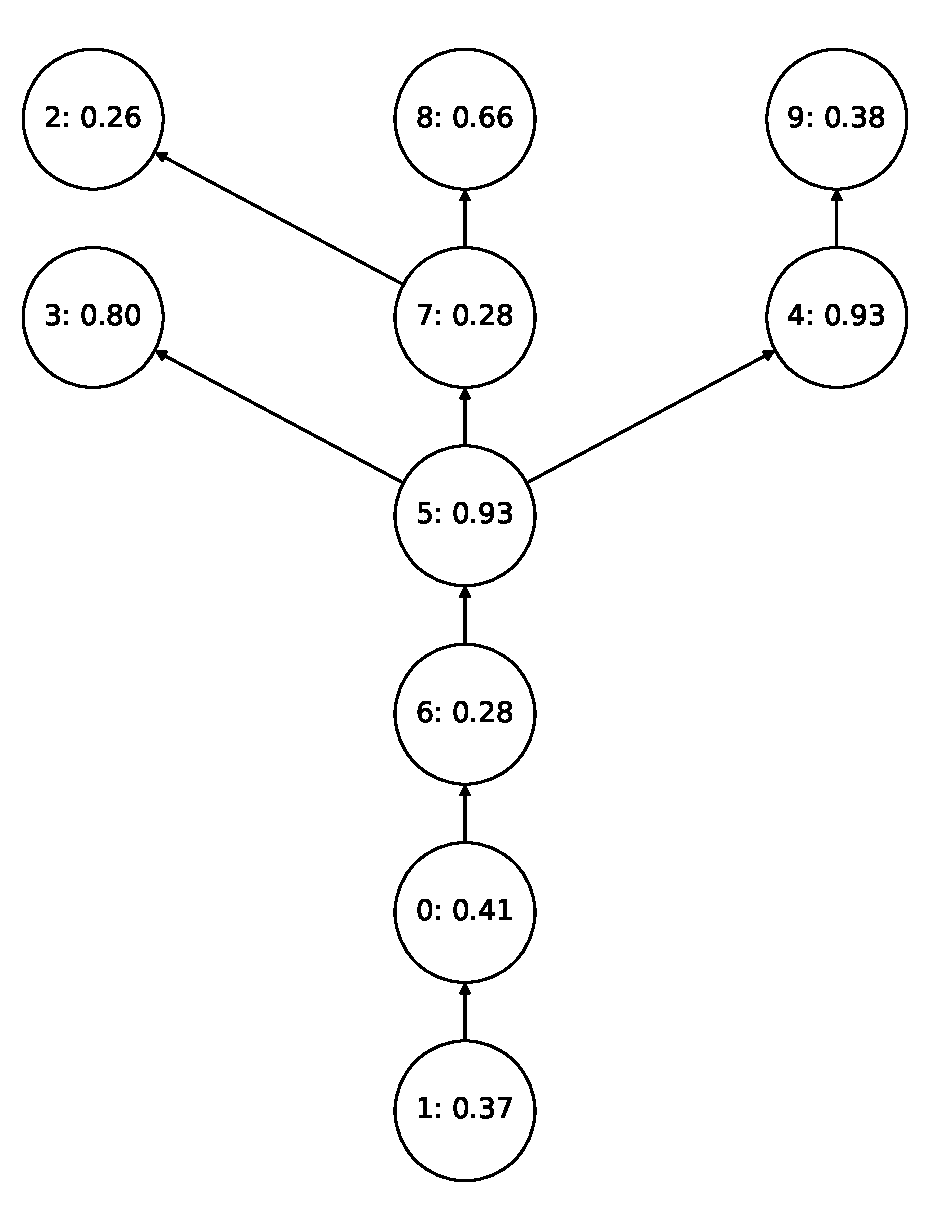
\includegraphics[width=\textwidth]{figures/computed/tree_10.pdf}
            \caption{Input tree of size 10.}
        \end{minipage}
        \begin{minipage}[t]{0.49\textwidth}
            \centering
            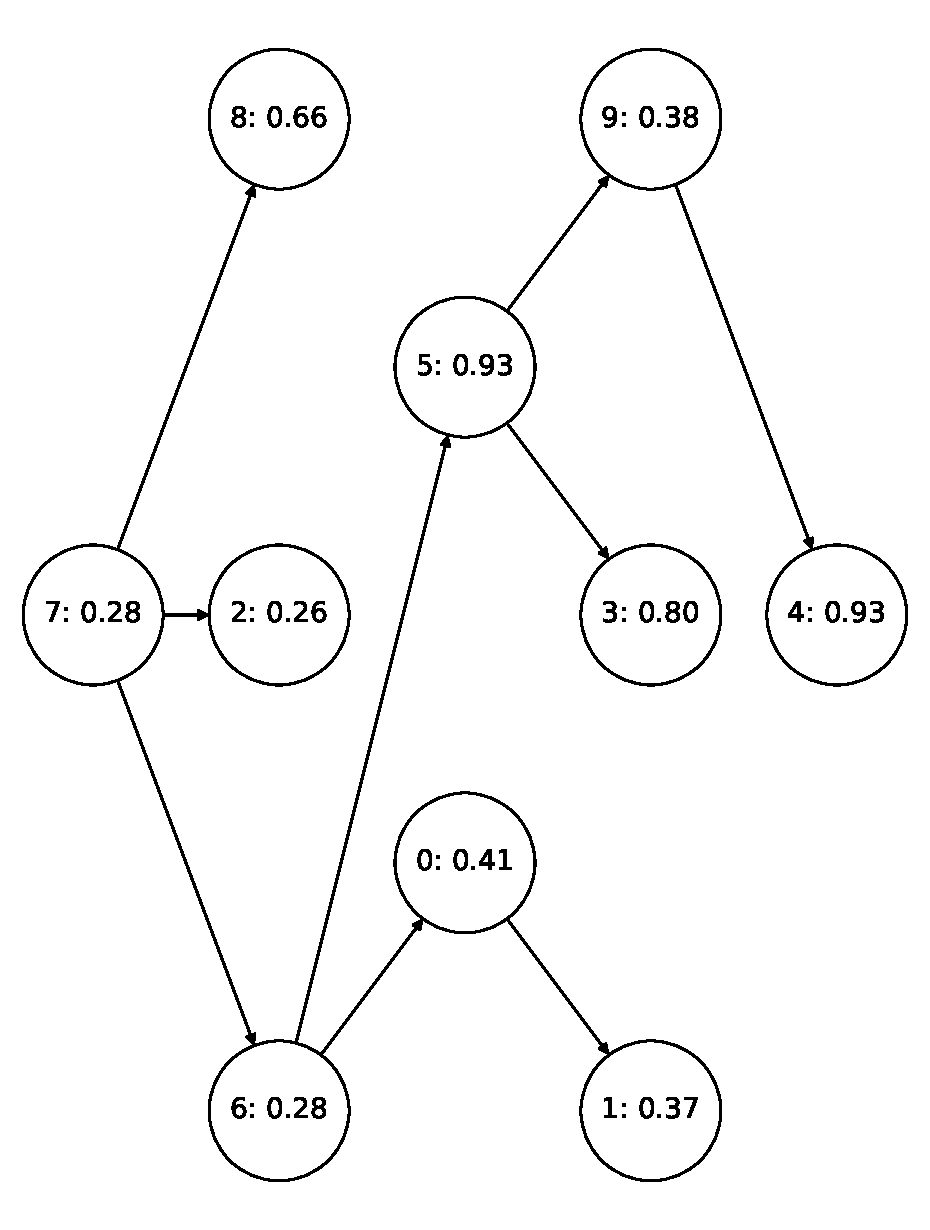
\includegraphics[width=\textwidth]{figures/computed/dt_10.pdf}
            \caption{Decision tree of cost 2.8.}
        \end{minipage}
        }
    \end{figure}

    \begin{figure}[htp]
        \scalebox{0.90}{
        \begin{minipage}[t]{0.49\textwidth}
            \centering
            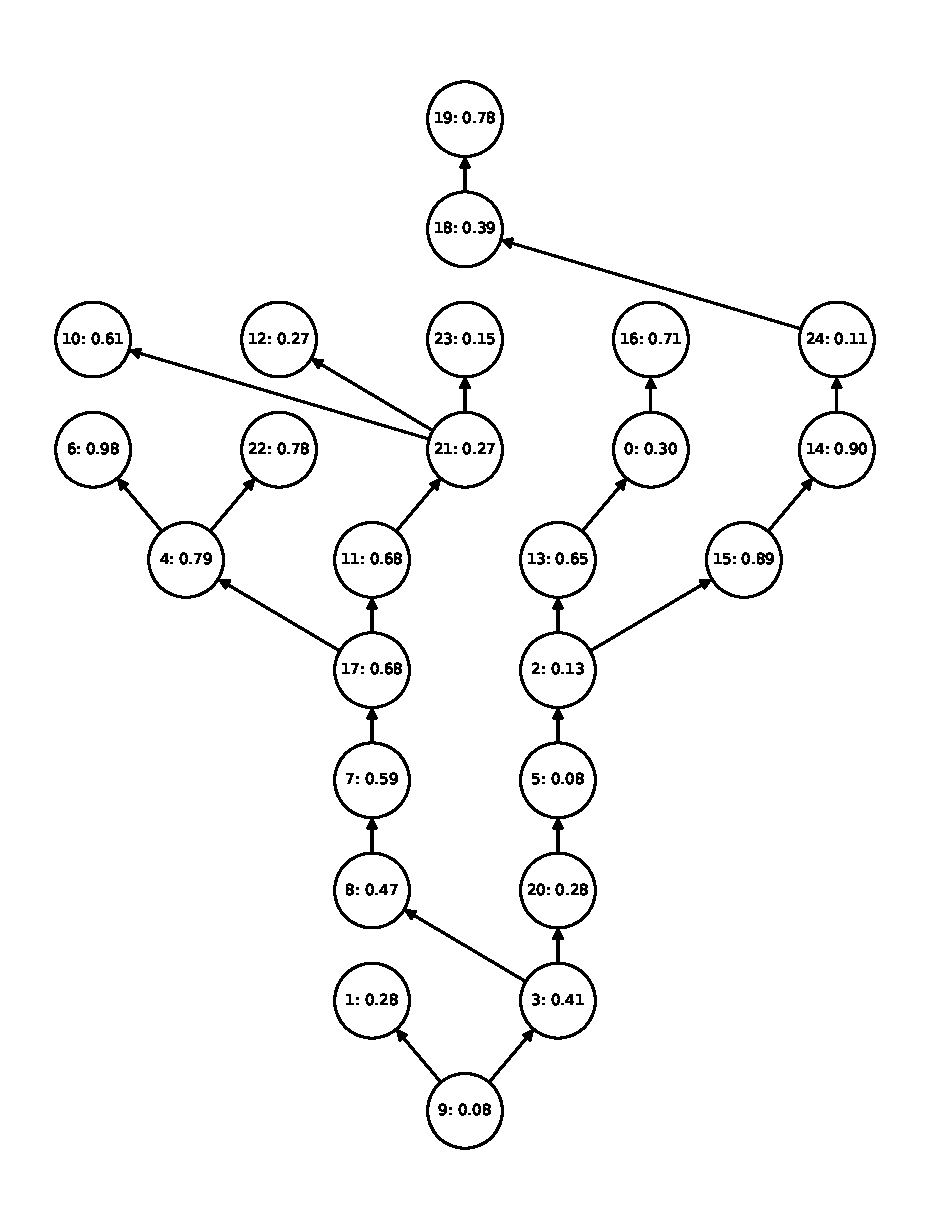
\includegraphics[width=\textwidth]{figures/computed/tree_25.pdf}
            \caption{Input tree of size 25.}
        \end{minipage}
        \begin{minipage}[t]{0.49\textwidth}
            \centering
            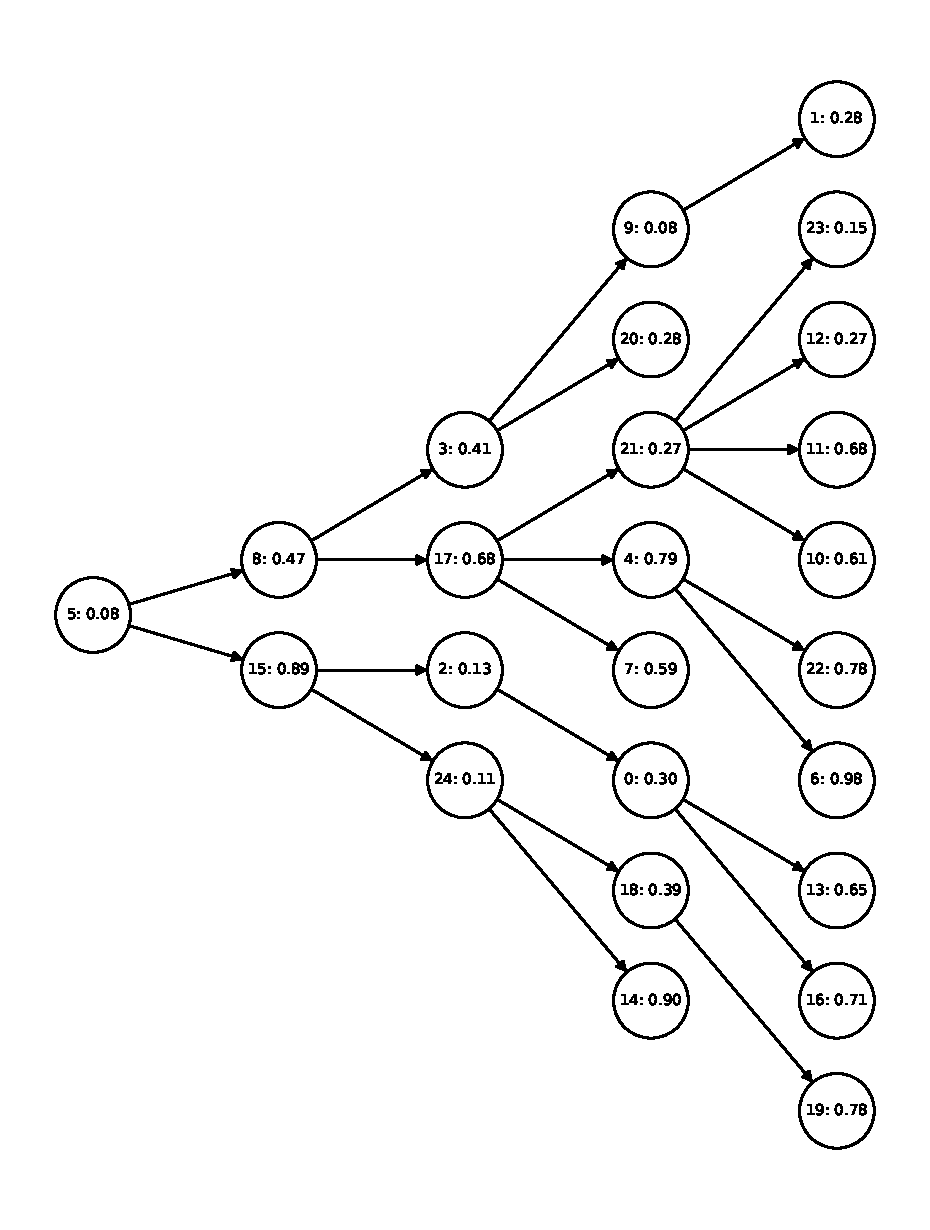
\includegraphics[width=\textwidth]{figures/computed/dt_25.pdf}
            \caption{Decision tree of cost 3.}
        \end{minipage}
        }
    \end{figure}

    \begin{figure}[htp]
        \scalebox{0.90}{
        \begin{minipage}[t]{0.49\textwidth}
            \centering
            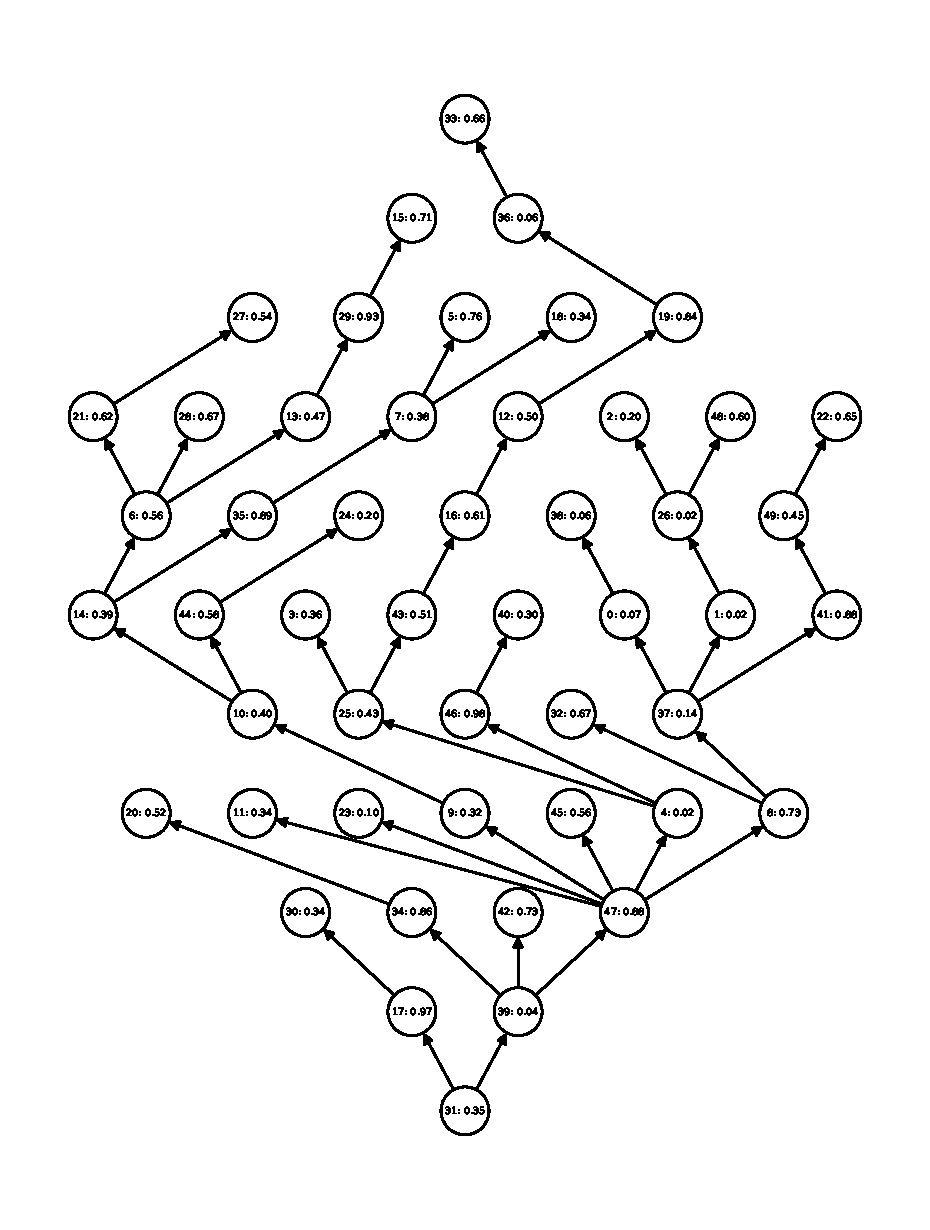
\includegraphics[width=\textwidth]{figures/computed/tree_50.pdf}
            \caption{Input tree of size 50.}
        \end{minipage}
        \begin{minipage}[t]{0.49\textwidth}
            \centering
            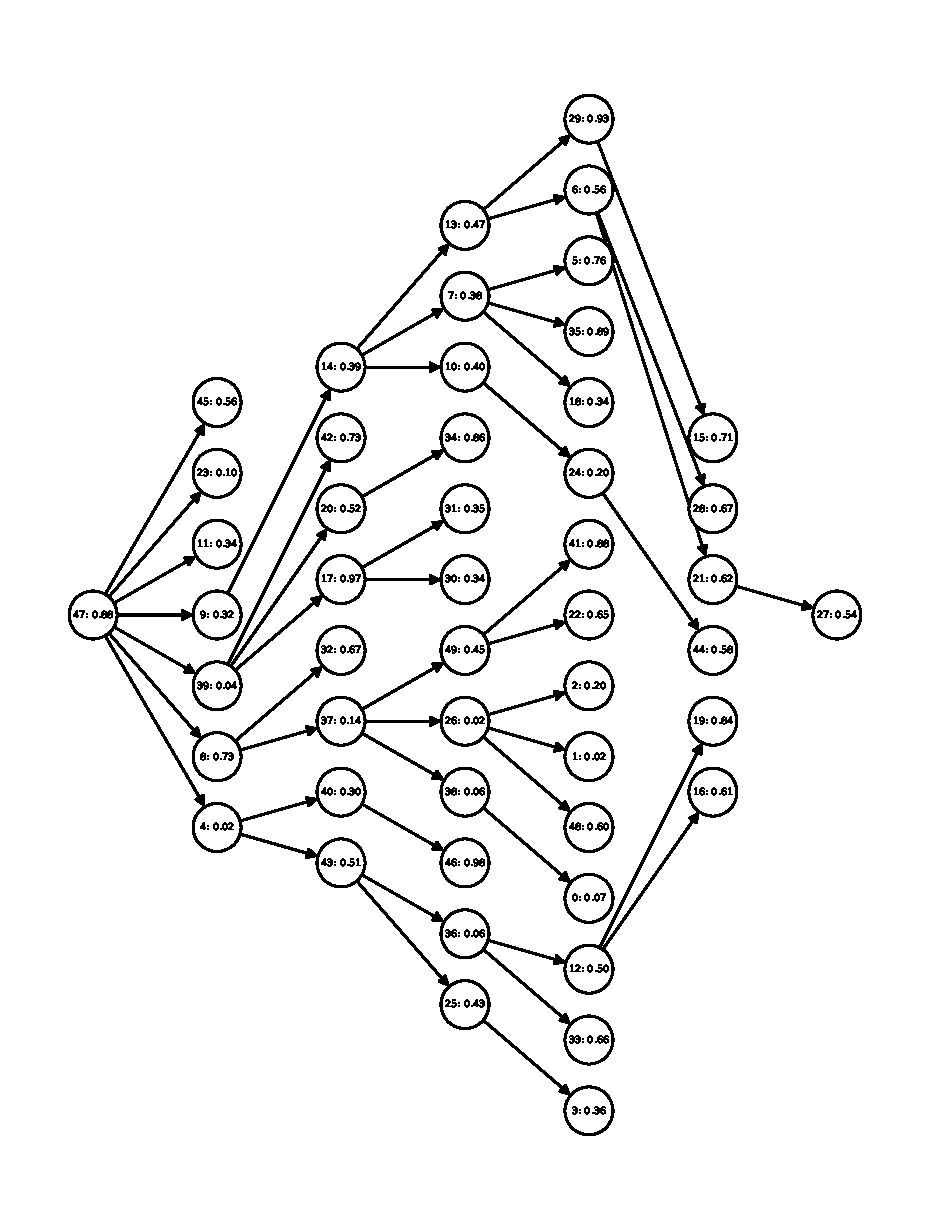
\includegraphics[width=\textwidth]{figures/computed/dt_50.pdf}
            \caption{Decision tree of cost 3.78.}
        \end{minipage}
        }
    \end{figure}

    \begin{figure}[htp]
        \scalebox{0.90}{
        \begin{minipage}[t]{0.49\textwidth}
            \centering
            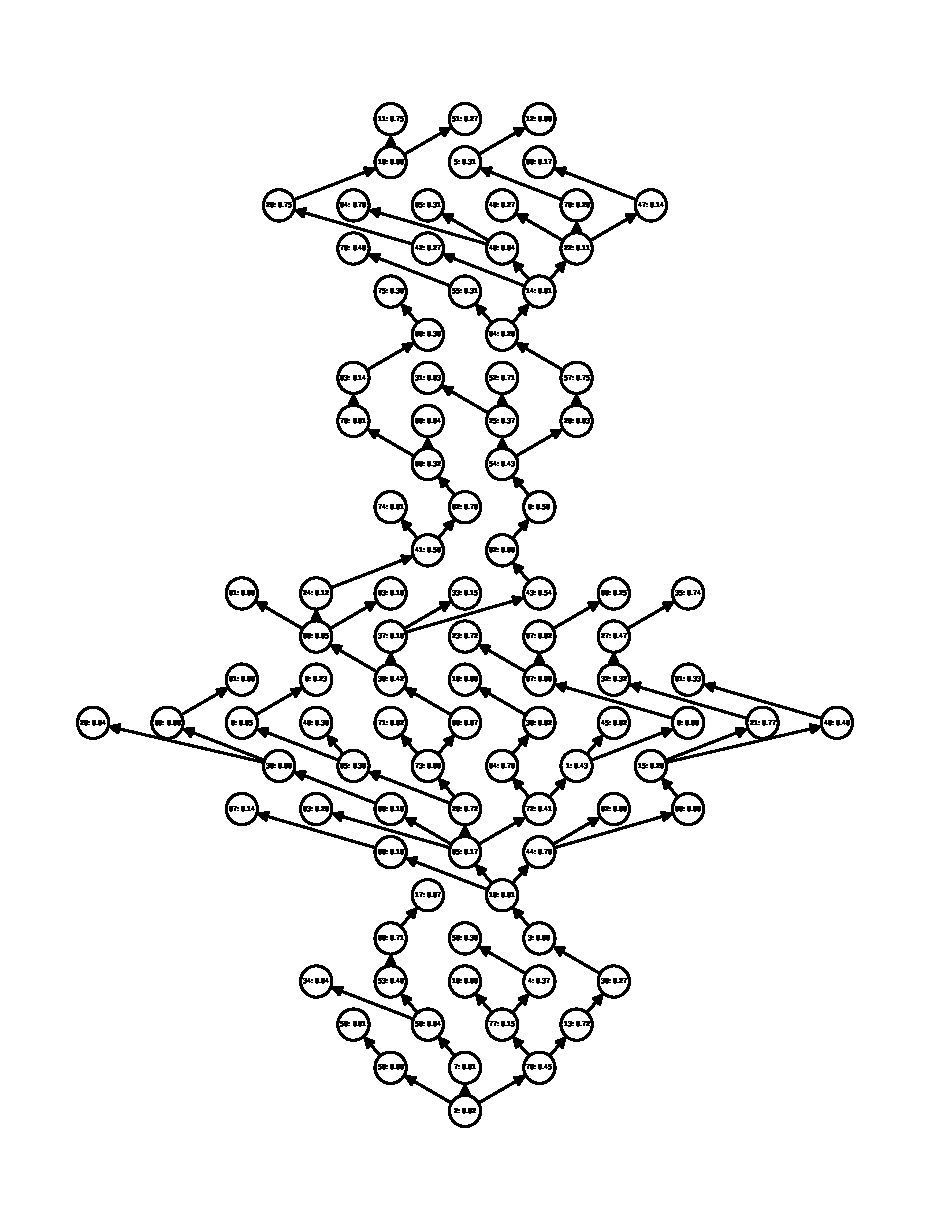
\includegraphics[width=\textwidth]{figures/computed/tree_100.pdf}
            \caption{Input tree of size 100.}
        \end{minipage}
        \begin{minipage}[t]{0.49\textwidth}
            \centering
            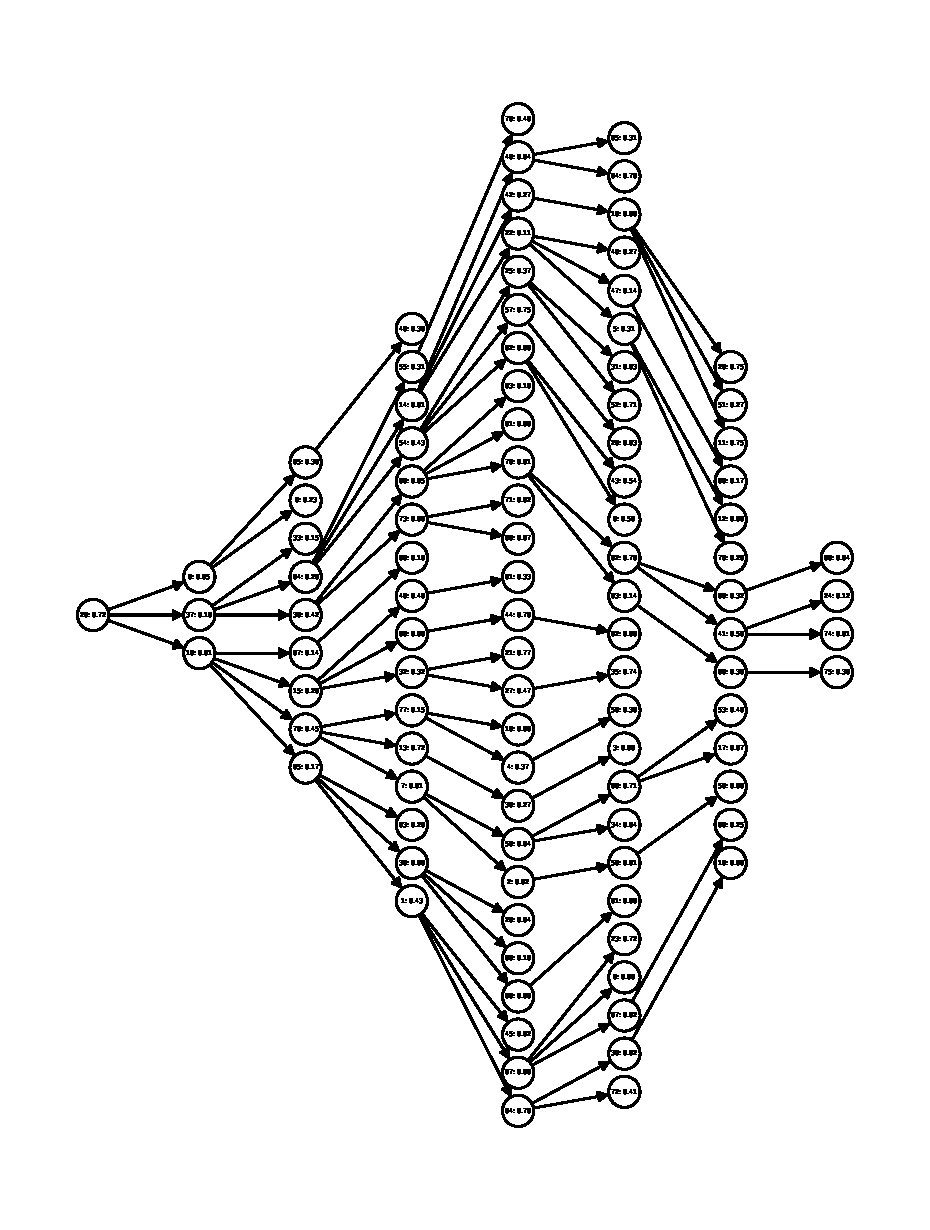
\includegraphics[width=\textwidth]{figures/computed/dt_100.pdf}
            \caption{Decision tree of cost 4.85.}
        \end{minipage}
        }
    \end{figure}
    \begin{figure}[htp]
        \scalebox{0.90}{
        \begin{minipage}[t]{0.49\textwidth}
            \centering
            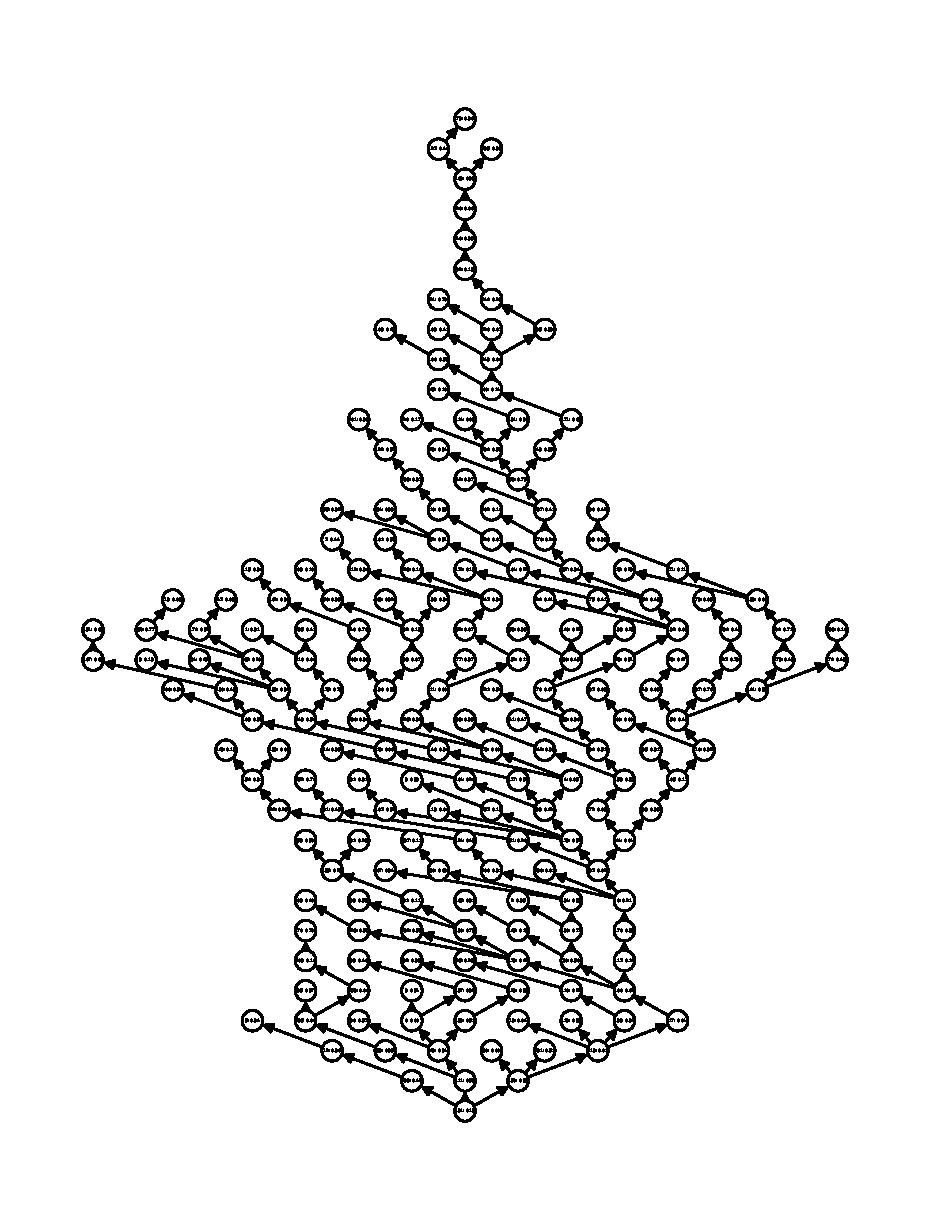
\includegraphics[width=\textwidth]{figures/computed/tree_200.pdf}
            \caption{Input tree of size 200.}
        \end{minipage}
        \begin{minipage}[t]{0.49\textwidth}
            \centering
            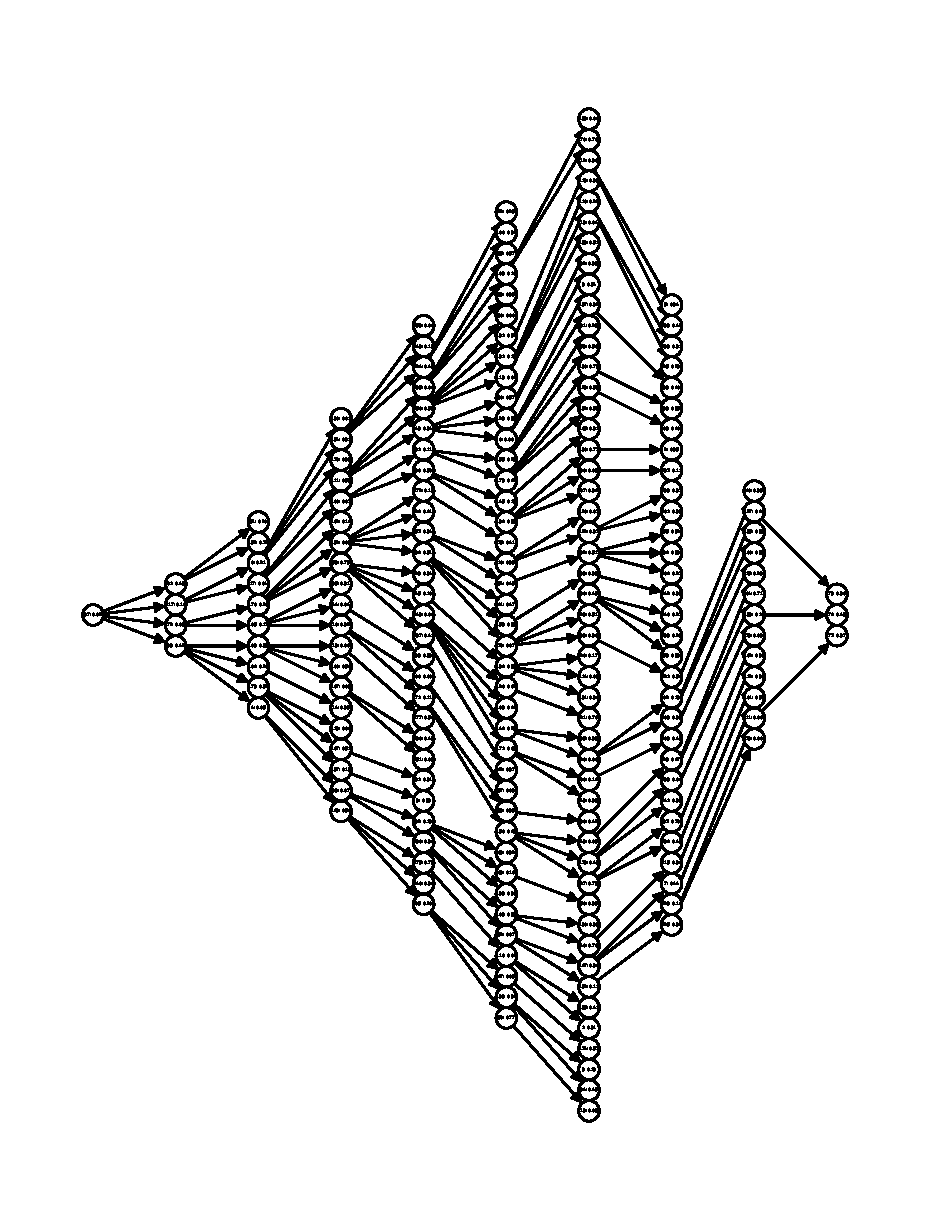
\includegraphics[width=\textwidth]{figures/computed/dt_200.pdf}
            \caption{Decision tree of cost 4.66}
        \end{minipage}
        }
    \end{figure}
\end{frame}

\begin{frame}{Basic steps}{}
\textbf{proc} $\FApproxDT\br{T}$:
\begin{enumerate}
    \item Set a global parameter $k=2^{\fl{\sqrt{\log n}}+2}$.
    \pause
    \item If $n\br{T}\leq k$, return $\FQPTAS\br{ T , \epsilon = 1}$.
    \pause
    \item Else, find a set $\mathcal{X}\subseteq V\br{ T }$, such that $\spr{\mathcal{X}}\leq k$ and for every $H\in T - \mathcal{X}$, $n\br{H}\leq n\br{ T }/2^{\sqrt{\log n}}$.
    \pause
    \item $\mathcal{Y}\gets \mathcal{X} \cup $ all branching vertices in $ T \angl{X}$.
    \item $\mathcal{Z}\gets \mathcal{Y}$ and all lightest vertices on paths between vertices of $Y$.
    \item $D\gets D_\mathcal{Z}\gets \FQPTAS\br{T_{\mathcal{Z}}, \epsilon = 1}$, where $ T _{\mathcal{Z}}$ is a tree built on $\mathcal{Z}$.
    \pause
    \item For every $H\in T - \mathcal{X}$, hang $D_H\gets\FApproxDT\br{H}$ in $D_{\mathcal{Z}}$.
    \item Return $D$.
\end{enumerate}
\end{frame}
\begin{frame}{Auxiliarry tree structure}
    
\begin{figure}[htp]
    \begin{minipage}[t]{0.45\textwidth}
    \centering
    \begin{tikzpicture}[every node/.style={draw, very thick}, every path/.style={very thick}]

    \node[circle, draw, minimum size=0.15cm, inner sep=0pt, fill=black] (27) at (-2.95,-1.95) {};
    
    \node[circle, draw, minimum size=0.15cm, inner sep=0pt, fill=black] (29) at (-0.5,-2) {};

    
    \node[circle, draw, minimum size=0.15cm, inner sep=0pt, fill=white] (30) at (1,-2.5) {};
    
    \node[circle, draw, minimum size=0.15cm, inner sep=0pt, fill=gray!55] (32) at (1.4,-3) {};

    \node[circle, draw, minimum size=0.15cm, inner sep=0pt, fill=black] (38) at (1.6,-2.79) {};
    \node[circle, draw, minimum size=0.15cm, inner sep=0pt, fill=white] (39) at (1.67,-3.025) {};
    
    \node[circle, draw, minimum size=0.15cm, inner sep=0pt, fill=white] (33) at (1.75,-3.5) {};
    
    \node[circle, draw, minimum size=0.15cm, inner sep=0pt, fill=black] (35) at (2.05,-3.95) {};
    
    \node[circle, draw, minimum size=0.15cm, inner sep=0pt, fill=black] (2) at (-3,3) {};

    
    
    \node[circle, draw, minimum size=0.15cm, inner sep=0pt, fill=black] (4) at (-0.85,2.5) {};
    
    \node[circle, draw, minimum size=0.15cm, inner sep=0pt, fill=white] (5) at (-2.77,2) {};
    
    \node[circle, draw, minimum size=0.15cm, inner sep=0pt, fill=white] (6) at (-0.7,1.25) {};
    ;
    \node[circle, draw, minimum size=0.15cm, inner sep=0pt, fill=black] (8) at (1.75,0.95) {};
    
    \node[circle, draw, inner sep=0pt, fill=white] (9) at (-2.53,1) {};
    
    \node[circle, draw, minimum size=0.15cm, inner sep=0pt, fill=white] (10) at (1,0.65) {};
    
    \node[circle, draw, inner sep=0pt, fill=white] (11) at (0.5,0.47) {};
    
    \node[circle, draw, minimum size=0.15cm, inner sep=0pt, fill=gray!55] (12) at (-0.52,0.1) {};
    
    \node[circle, draw, minimum size=0.15cm, inner sep=0pt, fill=white] (13) at (-0.95,-0.1) {};

    
    \node[circle, draw, minimum size=0.15cm, inner sep=0pt, fill=black] (15) at (-2.2,-0.4) {};
    \node[circle, draw, minimum size=0.15cm, inner sep=0pt, fill=white] (16) at (-2,-0.45) {};
    \node[circle, draw, minimum size=0.15cm, inner sep=0pt, fill=gray!55] (17) at (-1.8,-0.5) {};
    
    \node[circle, draw, minimum size=0.15cm, inner sep=0pt, fill=white] (18) at (-1.35,-1.1) {};

    \node[circle, draw, minimum size=0.15cm, inner sep=0pt, fill=white] (19) at (-2.4,-1.25) {};
    
    \node[circle, draw, inner sep=0pt, fill=white] (20) at (-1.05,-1.45) {};
    
    \node[circle, draw, minimum size=0.15cm, inner sep=0pt, fill=black] (22) at (1.5,-1.55) {};
    
    \node[circle, draw, minimum size=0.15cm, inner sep=0pt, fill=white] (23) at (1,-1.65) {};
    
    \node[circle, draw, minimum size=0.15cm, inner sep=0pt, fill=gray!55] (24) at (0.5,-1.775) {};
    
    \node[circle, draw, minimum size=0.15cm, inner sep=0pt, fill=white] (25) at (0.25,-1.85) {};

    
    
    \draw[] (2) to (5);
    \draw[] (4) to (6);
    \draw[] (5) to (9);
    \draw[] (6) to (12);
    \draw[] (8) to (10);
    \draw[] (9) to (15);
    \draw[] (10) to (11);
    \draw[] (11) to (12);
    \draw[] (12) to (13);
    \draw[] (13) to (17);
    \draw[] (15) to (16);
    \draw[] (16) to (17);
    \draw[] (17) to (18);
    \draw[] (17) to (19);
    \draw[] (18) to (20);
    \draw[] (19) to (27);
    \draw[] (20) to (29);
    \draw[] (22) to (23);
    \draw[] (23) to (24);
    \draw[] (24) to (25);
    \draw[] (24) to (30);
    \draw[] (25) to (29);
    \draw[] (30) to (32);
    \draw[] (32) to (33);
    \draw[] (32) to (39);
    \draw[] (33) to (35);
    \draw[] (38) to (39);

    \draw[very thick, fill=gray!20, drop shadow]
    (2).. controls +(-40:2.5cm) and +(40:2.5cm).. (2);

    \draw[very thick, fill=gray!20, drop shadow]
    (9).. controls +(-120:1.5cm) and +(-200:1.5cm).. (9);

    \draw[very thick, fill=gray!20, drop shadow]
    (11).. controls +(-50:3cm) and +(-130:3cm).. (11);

    \draw[very thick, fill=gray!20, drop shadow]
    (20).. controls +(-105:2cm) and +(-185:2cm).. (20);

    \draw[very thick, fill=gray!20, drop shadow]
    (4).. controls +(30:3cm) and +(-50:3cm).. (4);

    \draw[very thick, fill=gray!20, drop shadow]
    (32).. controls +(-80:2cm) and +(-160:2cm).. (32);

    \draw[very thick, fill=gray!20, drop shadow]
    (4).. controls +(-100:1.75cm) and +(-180:1.75cm).. (4);

    \draw[very thick, fill=gray!20, drop shadow]
    (8).. controls +(180:1.5cm) and +(100:1.5cm).. (8);

     \draw[very thick, fill=gray!20, drop shadow]
    (10).. controls +(0:2.5cm) and +(-80:2.5cm).. (10);


    \draw[very thick, fill=gray!20, drop shadow]
    (15).. controls +(-200:1.5cm) and +(-120:1.5cm).. (15);

    \draw[very thick, fill=gray!20, drop shadow]
    (17).. controls +(125:1cm) and +(45:1cm).. (17);

    
    \draw[very thick, fill=gray!20, drop shadow]
    (22).. controls +(0:1.75cm) and +(-80:1.75cm).. (22);

     \draw[very thick, fill=gray!20, drop shadow]
    (27).. controls +(-20:3.5cm) and +(-100:3.5cm).. (27);

    
    \draw[very thick, fill=gray!20, drop shadow]
    (29).. controls +(-40:3cm) and +(-120:3cm).. (29);

    \draw[very thick, fill=gray!20, drop shadow]
    (29).. controls +(120:1.5cm) and +(30:1.5cm).. (29);

    \draw[very thick, fill=gray!20, drop shadow]
    (35).. controls +(-40:1cm) and +(-120:1cm).. (35);

    \draw[very thick, fill=gray!20, drop shadow]
    (38).. controls +(-20:0.8cm) and +(60:0.8cm).. (38);

    
    \end{tikzpicture}
    \caption[Example tree $\mathcal{T}$ with sets $\mathcal{X},\mathcal{Y},\mathcal{Z}$]{Example tree $\mathcal{T}$. Light grey regions represent light subtrees. Black vertices represent $\mathcal{X}$. Gray and black vertices represent $\mathcal{Y}$. White, gray and black vertices represent $\mathcal{Z}$. Lines represent paths of vertices between vertices of $\mathcal{Z}$.}\label{exampleTreeWithSetZcicalese}
\end{minipage}
    \hspace{0.06\textwidth} % Add space between the two minipages
    \begin{minipage}[t]{0.45\textwidth}
    \centering
    \begin{tikzpicture}[every node/.style={draw, very thick, drop shadow}, every path/.style={very thick}]
    
    \node[circle, draw, minimum size=0.3cm, inner sep=0pt, fill=black] (2) at (-3,4) {};

    
    
    \node[circle, draw, minimum size=0.3cm, inner sep=0pt, fill=black] (4) at (-0.85,3.5) {};
    

    
    \node[circle, draw, minimum size=0.3cm, inner sep=0pt, fill=white] (5) at (-2.77,3) {};
    
    \node[circle, draw, minimum size=0.3cm, inner sep=0pt, fill=white] (6) at (-0.7,2.25) {};
    
    \node[circle, draw, minimum size=0.3cm, inner sep=0pt, fill=black] (8) at (2,2) {};
    
    
    \node[circle, draw, minimum size=0.3cm, inner sep=0pt, fill=white] (10) at (1,1.65) {};
    
    
    \node[circle, draw, minimum size=0.3cm, inner sep=0pt, fill=gray!55] (12) at (-0.52,1.1) {};
    
    \node[circle, draw, minimum size=0.3cm, inner sep=0pt, fill=white] (13) at (-0.95,0.9) {};

    
    \node[circle, draw, minimum size=0.3cm, inner sep=0pt, fill=black] (15) at (-2.5,0.6) {};
    \node[circle, draw, minimum size=0.3cm, inner sep=0pt, fill=white] (16) at (-2,0.55) {};
    \node[circle, draw, minimum size=0.3cm, inner sep=0pt, fill=gray!55] (17) at (-1.5,0.5) {};
    
    \node[circle, draw, minimum size=0.3cm, inner sep=0pt, fill=white] (18) at (-1.35,-0.1) {};

    \node[circle, draw, minimum size=0.3cm, inner sep=0pt, fill=white] (19) at (-2.4,-0.25) {};
    
    
    \node[circle, draw, minimum size=0.3cm, inner sep=0pt, fill=black] (22) at (1.5,-0.55) {};
    
    \node[circle, draw, minimum size=0.3cm, inner sep=0pt, fill=white] (23) at (1,-0.65) {};
    
    \node[circle, draw, minimum size=0.3cm, inner sep=0pt, fill=gray!55] (24) at (0.5,-0.775) {};
    
    \node[circle, draw, minimum size=0.3cm, inner sep=0pt, fill=white] (25) at (0,-0.85) {};

    \node[circle, draw, minimum size=0.3cm, inner sep=0pt, fill=black] (27) at (-2.95,-0.95) {};
    
    \node[circle, draw, minimum size=0.3cm, inner sep=0pt, fill=black] (29) at (-0.5,-1) {};

    
    \node[circle, draw, minimum size=0.3cm, inner sep=0pt, fill=white] (30) at (1,-1.5) {};
    
    \node[circle, draw, minimum size=0.3cm, inner sep=0pt, fill=gray!55] (32) at (1.4,-2) {};
    \node[circle, draw, minimum size=0.3cm, inner sep=0pt, fill=black] (38) at (1.9,-1.55) {};
    \node[circle, draw, minimum size=0.3cm, inner sep=0pt, fill=white] (39) at (1.8,-1.95) {};
    
    \node[circle, draw, minimum size=0.3cm, inner sep=0pt, fill=white] (33) at (2,-2.5) {};
    
    \node[circle, draw, minimum size=0.3cm, inner sep=0pt, fill=black] (35) at (2.55,-2.95) {};
    
    \draw[] (2) to (5);
    \draw[] (4) to (6);
    \draw[] (5) to (15);
    \draw[] (6) to (12);
    \draw[] (8) to (10);
    \draw[] (10) to (12);
    \draw[] (12) to (13);
    \draw[] (13) to (17);
    \draw[] (15) to (16);
    \draw[] (16) to (17);
    \draw[] (17) to (18);
    \draw[] (17) to (19);
    \draw[] (18) to (29);
    \draw[] (19) to (27);
    \draw[] (22) to (23);
    \draw[] (23) to (24);
    \draw[] (24) to (25);
    \draw[] (24) to (30);
    \draw[] (25) to (29);
    \draw[] (30) to (32);
    \draw[] (32) to (33);
    \draw[] (32) to (39);
    \draw[] (33) to (35);
    \draw[] (38) to (39);
    \end{tikzpicture}
    \caption{Auxiliary tree $\mathcal{T}_{\mathcal{Z}}$ built from vertices of set $\mathcal{Z}$.}\label{exampleAuxTreeTZcicalese}
\end{minipage}
\begin{minipage}[t]{1\textwidth}
\centering
    \begin{tikzpicture}[scale=1.1]
    \draw[very thick, fill=gray, drop shadow] 
    (4,-3.4) -- (5.2,-5.8) -- (2.8,-5.8) -- cycle; 


    \draw[very thick, fill=gray!20, drop shadow] (2,-6.6) -- (2.9,-8.4) -- (1.1,-8.4) -- cycle;

    \draw[very thick, fill=gray!20, drop shadow] (4,-6.5) -- (4.8,-8.1) -- (3.2,-8.1) -- cycle;
    
    \node at (5.2, -7.3) {$\dots$}; 

    \draw[very thick, fill=gray!20, drop shadow] (6.4,-6.4) -- (5.7,-7.8) -- (7.1,-7.8) -- cycle;
    
    \draw[very thick] (2.8,-5.8) -- (2,-6.6);
    \draw[very thick] (4.2,-5.8) -- (4,-6.5);
    \draw[very thick] (5.2,-5.8) -- (6.4,-6.4);

    \draw [decorate, 
       decoration = {calligraphic brace, amplitude = 10pt, mirror}, 
       line width = 1.5pt] 
      (0.5,-3.25) -- (0.5,-8.45);

    \node at (-0.6, -5.85) {$\COST_{D}\br{\mathcal{T}}$};
        
    \end{tikzpicture}
    \caption[Auxiliary tree $\mathcal{T_{\mathcal{Z}}}$ construction and the structure of the decison tree $D_{\mathcal{Z}}$]{The structure of the decision tree $D$, built by the Algorithm \ref{cicalese_inspired_pseudocode}. The dark gray subtree represents the decision tree $D_{\mathcal{Z}}$, obtained by calling the \texttt{Exact} procedure for $\mathcal{T}_{\mathcal{Z}}$ and $c$. Light gray subtrees represent decision trees $D_L$, built for each $H\in \mathcal{T}-\mathcal{Z}$, by recursively calling \textsc{DecisionTree} with $H$ and $c$.}\label{structure_of_dt_cicalese}
\end{minipage}
\end{figure}
\end{frame}
\begin{frame}{Solution structure}
    
\begin{figure}[htp]
    \centering
    \scalebox{1}{
\begin{minipage}[t]{1\textwidth}
\centering
    \begin{tikzpicture}[]
    \draw[very thick, fill=gray, drop shadow] 
    (4,-3.4) -- (5.2,-5.8) -- (2.8,-5.8) -- cycle node[right] {$D_{\mathcal{Z}}$}; 


    \draw[very thick, fill=gray!20, drop shadow] (2,-6.6) -- (2.9,-8.4) -- (1.1,-8.4) -- cycle node[right] {$D_{H_1}$};

    \draw[very thick, fill=gray!20, drop shadow] (4,-6.5) -- (4.8,-8.1) -- (3.2,-8.1) -- cycle node[right] {$D_{H_2}$};
    
    \node at (5.2, -7.3) {$\dots$}; 

    \draw[very thick, fill=gray!20, drop shadow] (6.4,-6.4) -- (5.7,-7.8) -- (7.1,-7.8) -- cycle node[right] {$D_{H_p}$};
    
    \draw[very thick] (2.8,-5.8) -- (2,-6.6);
    \draw[very thick] (4.2,-5.8) -- (4,-6.5);
    \draw[very thick] (5.2,-5.8) -- (6.4,-6.4);

    \draw [decorate, 
       decoration = {calligraphic brace, amplitude = 10pt, mirror}, 
       line width = 1.5pt] 
      (0.5,-3.25) -- (0.5,-8.45);

    \node at (-0.75, -5.85) {$\COST_{D}\br{T}$};
        
    \end{tikzpicture}
    
    \caption{Structure of the decision tree $D$}
\end{minipage}
    }
\end{figure}
\end{frame}
\begin{frame}{Approximation guarantee}
Since $\COST_{D_\mathcal{Z}}\leq 2\cdot \OPT\br{T}$, we have:
\begin{align*}
    \COST_D\br{T} &\leq \COST_{D_\mathcal{Z}} + \max_{H\in T-\mathcal{Z}}\brc{\COST_{D_H}\br{H}}
    \\&\leq 
    2\cdot \log_{2^{\sqrt{\log n}}}\br{n}\cdot \OPT\br{T} 
    \\&=
     \frac{2\log n}{\sqrt{\log n}}\cdot \OPT\br{T} 
     \\&=
      2\sqrt{\log n}\cdot \OPT\br{T}.
\end{align*}
\end{frame}

\begin{frame}{Rounding trick}
    \begin{itemize}
        \item Let $p \in \mathbb{N}$,
        \item Let $k=a/pn$, for some $a\in \mathbb{N}$.
        \pause
        \item We define new cost function $c'$, called \textbf{aligned cost function}:

    $$
c'\br{v}=\begin{cases}
    \cl{c\br{c}}_k, & \text{if } c\br{v}>pk, \text{ \textit{heavy vertex}},\\
    \cl{c\br{c}}_{\frac{1}{pn}}, & \text{otherwise, \textit{light vertex}}.\\
\end{cases}
$$
    \end{itemize}
\end{frame}

\begin{frame}{Lemmas}
     
\begin{lemma}\label{rounded_dt_lemma}
    $
    \OPT\br{T,c'}\leq \br{1+\frac{2}{p}}\cdot \OPT\br{T,c}.
    $
\end{lemma}
\pause
\begin{lemma}\label{aligned_dts_lemma}
    There exists a decision tree $D$ for $\br{T,c'}$, such that:
    \begin{enumerate}
        \item $\COST_{D}\br{T, c'}\leq \br{1+\frac{3}{p}}\cdot\OPT\br{T, c'}$
        \item Starting point of each heavy query is aligned to a multiple of $c$,
        \item Starting point of each light query is aligned to a multiple of $\frac{1}{pn}$.
    \end{enumerate}
\end{lemma}
\pause

We call a decision tree fulfiling the requirements 2. and 3. of the above lemma an \textbf{aligned decision tree}.
\end{frame}

\begin{frame}{Aligned cost}

    For any vertex $v\in V\br{T}$ and query $q\in Q_{D}\br{T,v}$ the \textbf{contribution} $\kappa_{T,c,k}\br{q,v}$ of $u$ is defined as:

    $$
\kappa_{T,c}\br{q, v}= \begin{cases}
    0, & \text{if its a light down response},\\
    c\br{q}, & \text{otherwise}.
\end{cases}
$$
\pause
Then, the \textbf{aligned cost} of $D$ is defined as:

$$
\COST'_D\br{T,c',k}=\max_{v\in V\br{T}}\brc{\sum_{q\in Q_D\br{T,v}}\kappa_{T,c', k}\br{q,v}}.
$$

Let $\OPT'\br{T,c',k}$ denote the optimal aligned cost.
\end{frame}
\begin{frame}{Heavy module contraction}

\begin{figure}[htbp]
    \begin{minipage}[t]{0.5\textwidth}
    \centering
    \begin{tikzpicture}[every node/.style={draw, very thick}, every path/.style={very thick}]
    
    \draw[dashed, thick, rounded corners = 10pt, fill= gray!25]
         (-1.25,5.75)  -- (-0.5,5.85)--  (-0.45,5.1) -- (-1.1,5.05) -- cycle;

    \draw[dashed, thick, rounded corners = 18pt, fill= gray!25]
        (0.45,5.8)  -- (1.7,5.8)-- (3.95,4.37) -- (2.6,4.05) -- (-0.7,4.1) -- cycle;
    \draw[dashed, thick, rounded corners = 9pt, fill= gray!25]
        (-2.1,2.6) -- (-1.7,2.95) -- (-1.2,2.8)  -- (-1.5,2.1) -- cycle;
        
    \draw[dashed, thick, rounded corners = 15pt, fill= gray!25]
         (-0.6,2.65) -- (0.25,3.1) -- (1.4,1.28) -- (-1.4,1.2) -- cycle;

    \draw[dashed, thick, rounded corners = 9pt, fill= gray!25]
        (1.9,2.8)  -- (2.55,3)  -- (2.9,2.6) -- (2.3,2.1) -- cycle;
    
    \node[circle, draw, fill=white] (1) at (0,6.4) {};
    
    \node[circle, draw, fill=black] (2) at (-0.8,5.44) {};
    \node[circle, draw, fill=black] (3) at (0.8,5.44) {};

    \node[circle, draw, fill=white] (4) at (-1.6,4.48) {};
    \node[circle, draw, fill=black] (5) at (0,4.48) {};
    \node[circle, draw, fill=black] (6) at (2.0,4.48) {};
    \node[circle, draw, fill=black] (7) at (3.2,4.48) {};
    
    \node[circle, draw, fill=white] (8) at (-0.8,3.52) {};
    \node[circle, draw, fill=white] (9) at (0.4,3.52) {};
    \node[circle, draw, fill=white] (10) at (1.6,3.52) {};
    \node[circle, draw, fill=white] (11) at (2.8,3.52) {};
    
    \node[circle, draw, fill=black] (12) at (-1.6,2.56) {};
    \node[circle, draw, fill=black] (13) at (0,2.56) {};
    \node[circle, draw, fill=black] (14) at (2.4,2.56) {};
    
    \node[circle, draw, fill=black] (15) at (-0.8,1.6) {};
    \node[circle, draw, fill=black] (16) at (0.8,1.6) {};
    \node[circle, draw, fill=white] (17) at (3.2,1.6) {};
    
    \node[circle, draw, fill=white] (18) at (0,0.64) {};
    \node[circle, draw, fill=white] (19) at (1.6,0.64) {};
    
    \draw[bend right=5] (1) to (2);
    \draw[bend left=5] (1) to (3);
    
    \draw[bend right=5] (2) to (4);
    \draw[bend right=5] (3) to (5);
    \draw[bend left=5] (3) to (6);
    \draw[bend left=5] (3) to (7);
    
    \draw[bend right=5] (5) to (8);
    \draw[bend left=5] (5) to (9);
    \draw[bend right=5] (6) to (10);
    \draw[bend left=5] (6) to (11);
    
    \draw[bend right=5] (8) to (12);
    \draw[bend left=5] (8) to (13);
    \draw[bend left=5] (10) to (14);
    
    \draw[bend right=5] (13) to (15);
    \draw[bend left=5] (13) to (16);
    \draw[bend left=5] (14) to (17);
    
    \draw[bend right=5] (16) to (18);
    \draw[bend left=5] (16) to (19);

    \end{tikzpicture}
\end{minipage}
    \begin{minipage}[t]{0.5\textwidth}
    \centering
    \begin{tikzpicture}[every node/.style={draw,rounded corners=5pt, very thick}, every path/.style={very thick}]
    
    \node[rectangle, minimum size=0.75cm, draw] (1) at (-0.56,10) {};
    
    \node[circle, draw] (2) at (-2.24,8) {};
    \node[rectangle, minimum size=0.75cm, draw] (3) at (-1.12,8) {};
    \node[circle, draw] (4) at (0,8) {};
    \node[rectangle, minimum size=0.75cm, draw] (5) at (1.12,8) {};
    \node[circle, draw] (6) at (2.24,8) {};
    
    \node[circle, draw] (7) at (-1.8,6) {};
    \node[circle, draw] (8) at (-0.56,6) {};
    \node[circle, draw] (9) at (1.8,6) {};
    
    \draw[bend right=5] (1) to (2);
    \draw[bend right=5] (1) to (3);
    \draw[bend left=5] (1) to (4);
    \draw[bend left=5] (1) to (5);
    \draw[bend left=5] (1) to (6);
    
    \draw[bend right=5] (3) to (7);
    \draw[bend left=5] (3) to (8);
    \draw[bend left=5] (5) to (9);

    \end{tikzpicture}
\end{minipage}
    \caption[Heavy module contraction]{Example of contracting 5 heavy modules. Black vertices represent heavy vertices, white vertices represent light vertices and square vertices represent vertices which were a parent of at least one heavy module before contraction.}\label{exampleHeavymoduleContraction}
\end{figure}
\end{frame}

\begin{frame}{Propositions}
\begin{block}{Proposition}
     Let $T$ be a tree, $c'$ an aligned cost function, $p\in \mathbb{N}$, $k$ the box size, $n$ the size of the original input tree, and $d$ be the depth. There exists a \FDPTimelinesCosts procedure which calculates an optimal aligned decision tree $D$, running in $pn^{O\br{d}}$ time.
    \end{block}
\pause 
\begin{block}{Proposition}
     Let $T$ be a tree, $c'$ be an aligned cost function, $D_A$ be a decision tree for $T$ and $F_C$ be forest of decision trees for $T$ with all heavy groups contracted, $p\in \mathbb{N}$ be a constant, $k\in \mathbb{R}_{>0}$ be the box size. There exists a polynomial time \FMergeDTs procedure which returns a decision tree of cost at most:
        $$
            \COST_{D}\br{T,c',k}=\OPT'\br{T,c',k}+2pk\cdot \COST_{F_C}\br{T,1}.
        $$
    \end{block}
\end{frame}

\begin{frame}{QPTAS}
\textbf{proc} $\FQPTAS\br{T, \epsilon}$:
\begin{enumerate}
    \item $p\gets \fl{35/\epsilon}$, 
    \item $d\gets p^2\cdot\br{\fl{\log n}+1}$.
    \item $k\gets 0$.
    \item Repeat the following steps until a decision tree $D$ is found:
    \begin{enumerate}
        \item $k\gets k +\frac{1}{pn}$.
        \item For every $v\in V\br{T}$, if $c\br{v}>pk$, then $c'\br{v}\gets\cl{c\br{v}}_k$, $c'\br{v}\gets\cl{c\br{v}}_{\frac{1}{pn}}$ otherwise.
        \item $D_A\gets \FDPTimelinesCosts\br{T,c',p,k,n,d}$
        \item If $D_A\neq\emptyset$:
        \begin{enumerate}
            \item $T_C\gets T$ with all heavy modules contracted.
        \item $D_C\gets \FRankingBasedDT\br{T_C}$.
        \item $D\gets \FMergeDTs\br{T, D_A, D_C}$.
        \end{enumerate}
    \end{enumerate}
    \item Return $D$.
\end{enumerate}
\end{frame}
\begin{frame}{Quality guarantee}
Let $k'$ be the value of $k$ for which $D$ was found. Since: $k'\leq \frac{\OPT'\br{T,c',k'}}{d}=\frac{\OPT'\br{T,c'}}{p^2\cdot\br{\fl{\log n}+1}}$, we have that:
\begin{align*}
    \COST_{D}\br{T,c'}&\leq \OPT'\br{T,c'}+2pk'\cdot \br{\fl{\log n}+1}
    \\&\leq 
    \OPT'\br{T,c'}+2p\cdot \br{\fl{\log n}+1}\cdot \frac{\OPT'\br{T,c'}}{p^2\cdot\br{\fl{\log n}+1}} \\
    & \leq \br{1+\frac{2}{p}}\cdot\OPT'\br{T,c'} 
    \\&\leq 
    \br{1+\frac{2}{p}}\cdot\br{1+\frac{2}{p}}\cdot\br{1+\frac{3}{p}}\cdot\OPT\br{T,c}
    \\&
    \leq \br{1+\frac{35}{p}}\cdot\OPT\br{T,c} 
    = 
    \br{1+\frac{35}{\cl{\frac{35}{\epsilon}}}}\cdot\OPT\br{T,c}
    \\&\leq 
    \br{1+\epsilon}\cdot \OPT\br{T,c}
\end{align*}
\end{frame}

% \begin{frame}{Medusa construction}
% 
\SetKwFunction{FDPTimelines}{DPTimelines}
\begin{figure}[htp]
\begin{minipage}[t]{1\textwidth}
    \centering
    \begin{tikzpicture}[every path/.style={very thick}]
    
    \node[text=white, circle, draw, minimum size=0.45cm, inner sep=0pt, fill=black] (1) at (0,0) {$a$};

    \node[text=white, circle, draw, minimum size=0.45cm, inner sep=0pt, fill=black] (2) at (-0.5,-1) {$b$};

    \node[text=white, circle, draw, minimum size=0.45cm, inner sep=0pt, fill=black] (3) at (0.5,-1) {$c$};

    \node[circle, draw, minimum size=0.45cm, inner sep=0pt, fill=white] (4) at (1.5,-1) {$d$};

    \draw[] (1) to (2);
    \draw[] (1) to (3);
    \draw[] (1) to (4);

    \node[text=white, circle, draw, minimum size=0.45cm, inner sep=0pt, fill=black] (5) at (-2,-2) {$e$};

    \node[text=white, circle, draw, minimum size=0.45cm, inner sep=0pt, fill=black] (6) at (-1,-2) {$f$};

    \node[circle, draw, minimum size=0.45cm, inner sep=0pt, fill=white] (7) at (0,-2) {$g$};

    \node[text=white, circle, draw, minimum size=0.45cm, inner sep=0pt, fill=black] (8) at (1,-2) {$h$};

    \node[circle, draw, minimum size=0.45cm, inner sep=0pt, fill=white] (9) at (2,-2) {$i$};

    \draw[] (2) to (5);
    \draw[] (2) to (6);

    \draw[] (3) to (7);
    \draw[] (3) to (8);

    \draw[] (4) to (9);

    \node[circle, draw, minimum size=0.45cm, inner sep=0pt, fill=white] (10) at (-1.5,-3) {$j$};

    \node[circle, draw, minimum size=0.45cm, inner sep=0pt, fill=white] (11) at (-0.5,-3) {$k$};

    \node[circle, draw, minimum size=0.45cm, inner sep=0pt, fill=white] (12) at (0.5,-3) {$l$};

    \node[text=white, circle, draw, minimum size=0.45cm, inner sep=0pt, fill=black] (13) at (1.5,-3) {$m$};

    \node[text=white, circle, draw, minimum size=0.45cm, inner sep=0pt, fill=black] (14) at (2.5,-3) {$n$};

    \node[circle, draw, minimum size=0.45cm, inner sep=0pt, fill=white] (15) at (3.5,-3) {$o$};

    \draw[] (6) to (10);

    \draw[] (7) to (11);
    \draw[] (7) to (12);

    \draw[] (8) to (13);

    \draw[] (9) to (14);
    \draw[] (9) to (15);

    \node[circle, draw, minimum size=0.45cm, inner sep=0pt, fill=white] (16) at (-2,-4) {$p$};

    \node[circle, draw, minimum size=0.45cm, inner sep=0pt, fill=white] (17) at (-1,-4) {$q$};

    \node[circle, draw, minimum size=0.45cm, inner sep=0pt, fill=white] (18) at (2,-4) {$r$};

    \node[circle, draw, minimum size=0.45cm, inner sep=0pt, fill=white] (19) at (3,-4) {$s$};

    \draw[] (10) to (16);
    
    \draw[] (11) to (17);
    
    \draw[] (14) to (18);
    \draw[] (14) to (19);

    \node[circle, draw, minimum size=0.45cm, inner sep=0pt, fill=white] (20) at (-1.5,-5) {$t$};

    \node[text=white, circle, draw, minimum size=0.45cm, inner sep=0pt, fill=black] (21) at (-0.5,-5) {$u$};

    \node[text=white, circle, draw, minimum size=0.45cm, inner sep=0pt, fill=black] (22) at (1.5,-5) {$v$};

    \draw[] (17) to (20);
    \draw[] (17) to (21);

    \draw[] (18) to (22);


    \node[circle, draw, minimum size=0.45cm, inner sep=0pt, fill=white] (23) at (-2,-6) {$w$};

    \node[circle, draw, minimum size=0.45cm, inner sep=0pt, fill=white] (24) at (-1,-6) {$x$};

    \node[circle, draw, minimum size=0.45cm, inner sep=0pt, fill=white] (25) at (0,-6) {$y$};

    \node[text=white, circle, draw, minimum size=0.45cm, inner sep=0pt, fill=black] (26) at (2,-6) {$z$};

    
    \draw[] (20) to (23);

    \draw[] (21) to (24);
    \draw[] (21) to (25);

    \draw[] (22) to (26);
    
    \end{tikzpicture}
    \caption[Input tree $T$ with a heavy root]{}\label{tree_h_root}
\end{minipage}
\begin{minipage}[t]{0.49\textwidth}
    \centering
    \begin{tikzpicture}[every path/.style={very thick}]
    
    \node[circle, draw, minimum size=0.45cm, inner sep=0pt, fill=white] (1) at (0,0) {$p$};

    \node[circle, draw, minimum size=0.45cm, inner sep=0pt, fill=white] (2) at (-0.5,-1) {$j$};

    \draw[] (1) to (2);

    \node[circle, draw, minimum size=0.45cm, inner sep=0pt, fill=white] (3) at (2,0) {$q$};



    \node[circle, draw, minimum size=0.45cm, inner sep=0pt, fill=white] (4) at (1.5,-1) {$l$};

    \node[circle, draw, minimum size=0.45cm, inner sep=0pt, fill=white] (5) at (2.5,-1) {$t$};

    \node[circle, draw, minimum size=0.45cm, inner sep=0pt, fill=white] (6) at (3.25,-1) {$x$};

    \node[circle, draw, minimum size=0.45cm, inner sep=0pt, fill=white] (7) at (4,-1) {$y$};

    

    \draw[] (3) to (4);
    \draw[] (3) to (5);
    \draw[] (3) to (6);
    \draw[] (3) to (7);

    \node[circle, draw, minimum size=0.45cm, inner sep=0pt, fill=white] (8) at (1,-2) {$g$};

    \node[circle, draw, minimum size=0.45cm, inner sep=0pt, fill=white] (9) at (3,-2) {$w$};

    \draw[] (4) to (8);
    \draw[] (5) to (9);

    \node[circle, draw, minimum size=0.45cm, inner sep=0pt, fill=white] (10) at (1.5,-3) {$w$};

    \draw[] (8) to (10);



    \node[circle, draw, minimum size=0.45cm, inner sep=0pt, fill=white] (11) at (-1,-2) {$r$};


    \node[circle, draw, minimum size=0.45cm, inner sep=0pt, fill=white] (12) at (-0.5,-3) {$o$};

    \draw[] (11) to (12);

    \node[circle, draw, minimum size=0.45cm, inner sep=0pt, fill=white] (13) at (0,-4) {$i$};

    \draw[] (12) to (13);

    \node[circle, draw, minimum size=0.45cm, inner sep=0pt, fill=white] (14) at (-0.5,-5) {$s$};

    \node[circle, draw, minimum size=0.45cm, inner sep=0pt, fill=white] (15) at (0.5,-5) {$d$};

    \draw[] (13) to (14);
    \draw[] (13) to (15);


    
    \end{tikzpicture}
    \caption[Input forest of decision trees for light vertices $F_C$.]{}\label{input_forest}
\end{minipage}
\begin{minipage}[t]{0.49\textwidth}
    \centering
    \begin{tikzpicture}[every path/.style={very thick}]
    
    \node[text=white, circle, draw, minimum size=0.45cm, inner sep=0pt, fill=black] (1) at (0,0) {$a$};

    \node[text=white, circle, draw, minimum size=0.45cm, inner sep=0pt, fill=black] (2) at (-0.5,-1) {$b$};

    \node[text=white, circle, draw, minimum size=0.45cm, inner sep=0pt, fill=black] (3) at (0.5,-1) {$c$};

    \node[circle, draw, minimum size=0.45cm, inner sep=0pt, fill=white] (4) at (1.5,-1) {$d$};

    \draw[] (1) to (2);
    \draw[] (1) to (3);
    \draw[] (1) to (4);

    \node[text=white, circle, draw, minimum size=0.45cm, inner sep=0pt, fill=black] (5) at (-2,-2) {$e$};

    \node[text=white, circle, draw, minimum size=0.45cm, inner sep=0pt, fill=black] (6) at (-1,-2) {$f$};

    \node[circle, draw, minimum size=0.45cm, inner sep=0pt, fill=white] (7) at (0,-2) {$g$};

    \node[text=white, circle, draw, minimum size=0.45cm, inner sep=0pt, fill=black] (8) at (1,-2) {$h$};

    \node[circle, draw, minimum size=0.45cm, inner sep=0pt, fill=white] (9) at (2,-2) {$i$};

    \draw[] (2) to (5);
    \draw[] (2) to (6);

    \draw[] (3) to (7);
    \draw[] (3) to (8);

    \draw[] (4) to (9);

    \node[circle, draw, minimum size=0.45cm, inner sep=0pt, fill=white] (10) at (-1.5,-3) {$j$};

    \node[circle, draw, minimum size=0.45cm, inner sep=0pt, fill=white] (11) at (-0.5,-3) {$q$};

    \node[circle, draw, minimum size=0.45cm, inner sep=0pt, fill=white] (12) at (0.5,-3) {$l$};

    \node[text=white, circle, draw, minimum size=0.45cm, inner sep=0pt, fill=black] (13) at (1.5,-3) {$m$};

    \node[circle, draw, minimum size=0.45cm, inner sep=0pt, fill=white] (14) at (2.5,-3) {$s$};

    \node[circle, draw, minimum size=0.45cm, inner sep=0pt, fill=white] (15) at (3.5,-3) {$o$};

    \draw[] (6) to (10);

    \draw[] (7) to (11);
    \draw[] (7) to (12);

    \draw[] (8) to (13);

    \draw[] (9) to (14);
    \draw[] (9) to (15);

    \node[circle, draw, minimum size=0.45cm, inner sep=0pt, fill=white] (16) at (-2,-4) {$p$};


    \draw[] (10) to (16);

    
    \end{tikzpicture}
    \caption[Medusa tree $T_M$]{}\label{medusa_tree}
\end{minipage}
\caption[Construction of the medusa tree]{Construction of the medusa tree. Figure \ref{tree_h_root} shows example input tree $T$ with a heavy root. Figure \ref{input_forest} shows example input forest of decision trees for light vertices $F_C$. Figure \ref{medusa_tree} shows the constructed medusa tree $T_M$.}\label{medusa_tree_construction_figure}
\end{figure}
% \end{frame}
\begin{frame}{\FMergeDTs procedure}
\textbf{proc} $\FMergeDTs\br{T, D_A}$:
\begin{enumerate}
    \item If $F_C$ is connected, $r=r\br{F_C}$.
    \item Else, $r=r\br{D_A}$.
    \item $D\gets$ decision tree with root $r$.
    \item For each $T'\in T-r$:
    \begin{enumerate}
        \item Let forest $F'_C$ be $F_C$ restricted to $T'_C$
        \item Let $D_A'$ be $D$ restricted to $T'$.
        \item $D'\gets \FMergeDTs\br{T', D_A', F'_C}$
        \item Hang $D'$ below $r$ in $D$.
    \end{enumerate}  
    \item Return $D$.
\end{enumerate}
\end{frame}
\begin{frame}{Boxed decision tree}
    \begin{definition}
        \textbf{Boxed decision tree}:
        \begin{enumerate}
        \item $D=\br{V\br{D}, E\br{D}, u, l}$, $V\br{D}$ - nodes of $D$, called \textit{boxes}, $E\br{D}$ - edges of $D$, $u:V\br{T}\times V\br{D}\to \brc{0, 1/pn,2/pn,\dots,k}$ - \textit{usage} function and $l:V\br{D}\to\brc{0, 1/pn,2/pn,\dots,k}$ - \textit{load} function.
        \pause
        \item For every $b\in V\br{D}$, $Q\br{b}=\brc{v\in V\br{T}|u\br{v,b}>0}$ - \textit{query assignment}, vertices of $T$, such that queries to them overlap with $b$.
        \pause
        \item All boxes containing $v$ form a left path. Additionally, for rach interior box $b$, $l\br{b}=0$ and $u\br{v,b}=k$.
        \pause
        \item For every $b\in V\br{D}$, $l\br{b}+\sum_{v\in V\br{T}}u\br{v,b}\leq k$ and for every $v\in V\br{T}$, either $\sum_{b\in V\br{D}}\br{v,b}=0$ or $\sum_{b\in V\br{D}}\br{v,b}=c'\br{v}$.
        \pause
        \item Every heavy query is aligned.
        \end{enumerate}  
    \end{definition}
\end{frame}
\begin{frame}
    
\SetKwFunction{FDPTimelines}{DPTimelines}
\begin{figure}[htp]
\begin{minipage}[t]{0.49\textwidth}
    \centering
    \begin{tikzpicture}[every path/.style={very thick}]

    \node[text=white, circle, draw, minimum size=0.45cm, inner sep=0pt, fill=black] (1) at (0,0) {$a$};

    \node[text=white, circle, draw, minimum size=0.45cm, inner sep=0pt, fill=black] (2) at (-0.5,-1) {$b$};

    \node[text=white, circle, draw, minimum size=0.45cm, inner sep=0pt, fill=black] (3) at (0.5,-1) {$c$};

    \node[circle, draw, minimum size=0.45cm, inner sep=0pt] (4) at (1.5,-1) {$d$};

    \draw[] (1) to (2);
    \draw[] (1) to (3);
    \draw[] (1) to (4);
    

    \node[text=white, circle, draw, minimum size=0.45cm, inner sep=0pt, fill=black] (5) at (-2,-2) {$e$};

    \node[text=white, circle, draw, minimum size=0.45cm, inner sep=0pt, fill=black] (6) at (-1,-2) {$f$};

    \node[circle, draw, minimum size=0.45cm, inner sep=0pt] (7) at (0,-2) {$g$};

    \node[text=white, circle, draw, minimum size=0.45cm, inner sep=0pt, fill=black] (8) at (1,-2) {$h$};

    \node[circle, draw, minimum size=0.45cm, inner sep=0pt] (9) at (2,-2) {$i$};

    \draw[] (2) to (5);
    \draw[] (2) to (6);

    \draw[] (3) to (7);
    \draw[] (3) to (8);

    \draw[] (4) to (9);

    \node[circle, draw, minimum size=0.45cm, inner sep=0pt] (10) at (-1.5,-3) {$j$};

    \node[circle, draw, minimum size=0.45cm, inner sep=0pt] (11) at (-0.5,-3) {$q$};

    \node[circle, draw, minimum size=0.45cm, inner sep=0pt] (12) at (0.5,-3) {$l$};

    \node[text=white, circle, draw, minimum size=0.45cm, inner sep=0pt, fill=black] (13) at (1.5,-3) {$m$};

    \node[circle, draw, minimum size=0.45cm, inner sep=0pt] (14) at (2.5,-3) {$s$};

    \node[circle, draw, minimum size=0.45cm, inner sep=0pt] (15) at (3.5,-3.05) {$o$};

    \draw[] (6) to (10);

    \draw[] (7) to (11);
    \draw[] (7) to (12);

    \draw[] (8) to (13);

    \draw[] (9) to (14);
    \draw[] (9) to (15);

    \node[circle, draw, minimum size=0.45cm, inner sep=0pt] (16) at (-2,-4) {$p$};


    \draw[] (10) to (16);

    
    \end{tikzpicture}
    \caption[Example tree $T$]{}\label{box_dt_input}
\end{minipage}
\begin{minipage}[t]{0.49\textwidth}
    \centering
    \begin{tikzpicture}[ every path/.style={thick}]
        \footnotesize
    \node[draw, 
        rounded corners=3pt, 
        minimum width=0.65cm, 
        minimum height=1.4cm, 
        align=center, fill=gray
        ] (A) at (0,-0.375) {\raisebox{0.7cm}{$c$}};

    \node[draw, 
        rounded corners=3pt, 
        minimum width=0.65cm, 
        minimum height=0.3cm, 
        align=center, fill=gray!20
        ] (A) at (0,-1.35) {$i$};
    
    \node[draw, 
        rounded corners=3pt, 
        minimum width=0.65cm, 
        minimum height=1.0cm, 
        align=center, fill=gray!20
        ] (A) at (0,-2.075) {$d$};

    \node[draw, 
        rounded corners=3pt, 
        minimum width=0.65cm, 
        minimum height=1.4cm, 
        align=center, fill=gray
        ] (A) at (0,-3.375) {\raisebox{0.7cm}{$b$}};

    \node[draw, 
        rounded corners=3pt, 
        minimum width=0.65cm, 
        minimum height=2.15cm, 
        align=center, fill=gray
        ] (A) at (0,-5.25) {\raisebox{1.4cm}{$a$}};

    \node[circle,  draw, dashed, rectangle, minimum size=0.75cm, inner sep=0pt] (11) at (0,0) {};

    \node[circle, draw, dashed, rectangle, minimum size=0.75cm, inner sep=0pt] (12) at (0,-0.75) {};

    \node[circle, draw, dashed, rectangle, minimum size=0.75cm, inner sep=0pt] (13) at (0,-1.5) {};

    \node[circle, draw, dashed, rectangle, minimum size=0.75cm, inner sep=0pt] (14) at (0,-2.25) {};

    \node[circle, draw, dashed, rectangle, minimum size=0.75cm, inner sep=0pt] (15) at (0,-3) {};

    \node[circle, draw, dashed, rectangle, minimum size=0.75cm, inner sep=0pt] (16) at (0,-3.75) {};

    \node[circle, draw, dashed, rectangle, minimum size=0.75cm, inner sep=0pt] (17) at (0,-4.5) {};

    \node[circle, draw, dashed, rectangle, minimum size=0.75cm, inner sep=0pt] (18) at (0,-5.25) {};
    
    \node[circle, draw, dashed, rectangle, minimum size=0.75cm, inner sep=0pt] (19) at (0,-6) {};

    \node[draw, 
        rounded corners=3pt, 
        minimum width=0.65cm, 
        minimum height=0.3cm, 
        align=center, fill=black
        ] (A) at (1,-2.075) {};
    
    \node[draw, 
        rounded corners=3pt, 
        minimum width=0.65cm, 
        minimum height=0.3cm, 
        align=center, fill=gray!20
        ] (A) at (1,-2.425) {$s$};
    
    \node[circle, draw, dashed, rectangle, minimum size=0.75cm, inner sep=0pt] (24) at (1,-2.25) {};

    \draw[] (13.east) to (24.north);

    \node[draw, 
        rounded corners=3pt, 
        minimum width=0.65cm, 
        minimum height=0.65cm, 
        align=center, fill=black
        ] (A) at (1,-4.5) {};

    \node[draw, 
        rounded corners=3pt, 
        minimum width=0.65cm, 
        minimum height=1.4cm, 
        align=center, fill=gray
        ] (A) at (1,-5.625) {\raisebox{0.7cm}{$e$}};

    \node[circle, draw, dashed, rectangle, minimum size=0.75cm, inner sep=0pt] (27) at (1,-4.5) {};

    \node[circle, draw, dashed, rectangle, minimum size=0.75cm, inner sep=0pt] (28) at (1,-5.25) {};
    
    \node[circle, draw, dashed, rectangle, minimum size=0.75cm, inner sep=0pt] (29) at (1,-6) {};

    \draw[] (16.east) to (27.north);

    \node[draw, 
        rounded corners=3pt, 
        minimum width=0.65cm, 
        minimum height=0.6cm, 
        align=center, fill=gray!20
        ] (A) at (2,-2.225) {$o$};
    
    \node[circle, draw, dashed, rectangle, minimum size=0.75cm, inner sep=0pt] (34) at (2,-2.25) {};

    \draw[] (13.east) to (34.north);

    \node[draw, 
        rounded corners=3pt, 
        minimum width=0.65cm, 
        minimum height=0.3cm, 
        align=center, fill=gray!20
        ] (A) at (2,-4.38) {$j$};
    
    \node[draw, 
        rounded corners=3pt, 
        minimum width=0.65cm, 
        minimum height=1.4cm, 
        align=center, fill=gray
        ] (A) at (2,-5.625) {\raisebox{0.7cm}{$f$}};

    \node[circle, draw, dashed, rectangle, minimum size=0.75cm, inner sep=0pt] (37) at (2,-4.5) {};

    \node[circle, draw, dashed, rectangle, minimum size=0.75cm, inner sep=0pt] (38) at (2,-5.25) {};
    
    \node[circle, draw, dashed, rectangle, minimum size=0.75cm, inner sep=0pt] (39) at (2,-6) {};

    \draw[] (16.east) to (37.north);

    
    \node[draw, 
        rounded corners=3pt, 
        minimum width=0.65cm, 
        minimum height=0.8cm, 
        align=center, fill=gray!20
        ] (A) at (3,-1.575) {\raisebox{0.3cm}{$q$}};

    \node[draw, 
        rounded corners=3pt, 
        minimum width=0.65cm, 
        minimum height=0.35cm, 
        align=center, fill=black
        ] (A) at (3,-2.212) {};


    \node[draw, 
        rounded corners=3pt, 
        minimum width=0.65cm, 
        minimum height=1.2cm, 
        align=center, fill=gray!20
        ] (A) at (3,-3.05) {$l$};

    \node[draw, 
        rounded corners=3pt, 
        minimum width=0.65cm, 
        minimum height=0.3cm, 
        align=center, fill=gray!20
        ] (A) at (3,-3.875) {$g$};

    \node[circle, draw, dashed, rectangle, minimum size=0.75cm, inner sep=0pt] (43) at (3,-1.5) {};

    \node[circle, draw, dashed, rectangle, minimum size=0.75cm, inner sep=0pt] (44) at (3,-2.25) {};
    
    \node[circle, draw, dashed, rectangle, minimum size=0.75cm, inner sep=0pt] (45) at (3,-3) {};

    \node[circle, draw, dashed, rectangle, minimum size=0.75cm, inner sep=0pt] (46) at (3,-3.75) {};

    \draw[] (12.east) to (43.north);

    \node[draw, 
        rounded corners=3pt, 
        minimum width=0.65cm, 
        minimum height=1.05cm, 
        align=center, fill=gray!20
        ] (A) at (3,-5.45) {\raisebox{0.5cm}{$p$}};

    \node[circle, draw, dashed, rectangle, minimum size=0.75cm, inner sep=0pt] (48) at (3,-5.25) {};
    
    \node[circle, draw, dashed, rectangle, minimum size=0.75cm, inner sep=0pt] (49) at (3,-6) {};

    \draw[] (37.east) to (48.north);

    \node[draw, 
        rounded corners=3pt, 
        minimum width=0.65cm, 
        minimum height=2.9cm, 
        align=center, fill=gray
        ] (A) at (4,-2.625) {\raisebox{0.7cm}{$m$}};

    \node[draw, 
        rounded corners=3pt, 
        minimum width=0.65cm, 
        minimum height=1.4cm, 
        align=center, fill=gray
        ] (A) at (4,-4.875) {\raisebox{0.7cm}{$h$}};

    \node[circle, draw, dashed, rectangle, minimum size=0.75cm, inner sep=0pt] (53) at (4,-1.5) {};

    \node[circle, draw, dashed, rectangle, minimum size=0.75cm, inner sep=0pt] (54) at (4,-2.25) {};

    \node[circle, draw, dashed, rectangle, minimum size=0.75cm, inner sep=0pt] (55) at (4,-3) {};

    \node[circle, draw, dashed, rectangle, minimum size=0.75cm, inner sep=0pt] (56) at (4,-3.75) {};

    \node[circle, draw, dashed, rectangle, minimum size=0.75cm, inner sep=0pt] (57) at (4,-4.5) {};

    \node[circle, draw, dashed, rectangle, minimum size=0.75cm, inner sep=0pt] (58) at (4,-5.25) {};
    
    \node[circle, draw, dashed, rectangle, minimum size=0.75cm, inner sep=0pt] (59) at (4,-6) {};

    \draw[] (12.east) to (53.north);
    
    \end{tikzpicture}
    \caption[Example boxed decision tree $D$]{}\label{box_dt}
\end{minipage}

\caption[Structure of a boxed decision tree]{Structure of a boxed decision tree. Figure \ref{box_dt_input} shows example input tree $T$, black vertices are heavy and white vertices are white. Figure \ref{box_dt} shows example boxed decision tree $D$ for $T$, dark gray queries are heavy, light gray queries are light, and black spaces represent additional load of boxes.}\label{box_dt_figure}
\end{figure}
\end{frame}
\begin{frame}{Boxline}
    \begin{definition}
        \textbf{Boxline}: $B=\angl{\br{b_1, \tau_1},\br{b_2, \tau_2},\dots, \br{b_d, \tau_d}}$, $b_j$ - box, such that $Q\br{b_j}=\emptyset$, $\tau_j$ - boolean flag. 
    \end{definition}
    \pause
    \begin{definition}
    \textbf{Left box-path} of $D$: 
    \begin{enumerate}
        \item $B_D=\angl{{q_1, f_1},\br{q_2, f_2},\dots, \br{q_h, f_h}}$, $q_j$ - box $f_j$ - boolean flag, obtained by traversing boxes of $D$ towards left. For each such box $b_j$, $q_j=l\br{b}+\sum_{v\in Q\br{b}}q\br{v, b}$, whereas $f_j$ denotes whether there exists a \textbf{transcending} query in $Q\br{b_j}$, i. e.: $v\in Q\br{b_j}$  such that $v\in Q\br{b_{j+1}}$.
        \item Decision tree$D$ with a left box-path $B_D$ is \textbf{box-compatible} with boxline $B$ ($h\leq d$), if $l\br{q_j}\geq l\br{b_j}$ and $\tau_j\implies f_j$.
    \end{enumerate}  
    \end{definition}
\end{frame}
\begin{frame}[allowframebreaks]{Useful operations}
\begin{itemize}
    \item Puting a query to vertex $v$ at $s$-th slot of a box $b$:
    \begin{enumerate}
        \item $\sigma\br{v}\gets c\br{v}$: 
        \item While $\sigma\br{v}>0$: 
        \begin{enumerate}
            \item $u\br{v, b}\gets\min\brc{k-s/pn, \sigma\br{v}}$.
            \item $\sigma\br{v}\gets \sigma\br{v}-u\br{v, b}$. 
            \item$b\gets$ left child of $b$.
        \end{enumerate}
    \end{enumerate} If such operation violates the definition of $D$ or query to $v$ transcendents any box $b_j$, such that $\tau_j$. we mark $D$ as \textbf{conflicted}. 
    \framebreak
    \item Bipartitioning of $B$. A bipartition of $B$ consists of $\br{B_1,B_2}$ such that:
    \begin{itemize}
        \item $\spr{B}=\spr{B_1}=\spr{B_2}$.
        \item $l\br{b_{1,j}}+l\br{b_{2,j}} - k = l\br{b_j}$.
        \item $\br{\tau_{1,j}\land \tau_{2,j} \iff \tau_{j}}$.
        \item$\br{\tau_{1,j}\lor \tau_{2,j}}$.
    \end{itemize} 
    \framebreak
    \item Rotating a decision tree $D$ around vertex $v$: 
    \begin{enumerate}
        \item $q_h\gets $ the box containing the end of the query to $v$.
        \item Sort vertices whose queries start in $Q\br{q_h}$ according to $c$.
        \item Create box $q$.
        \item Move queries from $Q\br{q_h}$ to $Q\br{q}$, so that all queries after $v$ are in $Q\br{q}$,
        \item Hang $q_h'$ as a right child of $q_h$.
        \item Rehang left child of $q_h$ as a left child of $q$. 
    \end{enumerate}
\end{itemize}
\end{frame}
\begin{frame}{Cases of DP}

\SetKwFunction{FDPTimelines}{DPTimelines}
\begin{figure}[htp]
\scalebox{0.65}{
\begin{minipage}[t]{0.24\textwidth}
    \centering
    \begin{tikzpicture}[every path/.style={very thick}]
    
    \node[circle, draw, minimum size=0.6cm, inner sep=0pt, fill=white] (1) at (0,0) {$v$};

    \draw[] (1) to (0.5,1);
    
    \node at (0.7,1.46) {\rotatebox{63.43}{$\dots$}}; 

    \path (0,0) ++(0,-2.8) node[draw=none] {};

    \end{tikzpicture}
    \caption[]{No children.}\label{no_children}
\end{minipage}
\begin{minipage}[t]{0.3\textwidth}
    \centering
    \begin{tikzpicture}[every path/.style={very thick}]
    
    \node[circle, draw, minimum size=0.6cm, inner sep=0pt, fill=white] (1) at (-1,0.5) {$v$};
    
    \draw[] (1) to (-0.5,1.5);
    
    \node at (-0.3,1.96) {\rotatebox{63.43}{$\dots$}}; 

    \draw[] (1) to (-1,-0.7);

    \footnotesize
    \draw[very thick, fill=gray!20, drop shadow] (-1,-0.7)  node[circle, draw, minimum size=0.6cm, inner sep=0pt, fill=white] {$c_{1}$} -- (-1.8,-2.3) -- (-0.2,-2.3) -- cycle;

    \path (0,0) ++(0,-2.35) node[draw=none] {};

    \end{tikzpicture}
    \caption[]{One child.}\label{one_child}
\end{minipage}
\begin{minipage}[t]{0.45\textwidth}
    \centering
    \begin{tikzpicture}[every path/.style={very thick}]
    
    
    \draw[dashed, thick, rounded corners = 18pt, fill= gray!30]
        (-2,-0.7)--(0.3,0.7)  -- (1.4,1.2) node[left] {$T_{v,i-1}$} --  (2.8,-2.5)  -- (-2.4,-2.3) -- cycle;


    \node[circle, draw, minimum size=0.6cm, inner sep=0pt, fill=white] (1) at (1,0.5) {$v$};

    \draw[] (1) to (1.5,1.5);
    
    \node at (1.7,1.96) {\rotatebox{63.43}{$\dots$}}; 
    
    \draw[] (1) to (-1.3,-1);
    \draw[] (1) to (0,-0.9);
    \draw[] (1) to (1.5,-0.8);

    \draw[] (1) to (4,-0.7);
    
    \footnotesize

    \draw[very thick, fill=gray!20, drop shadow] (-1.3,-1) node[circle, draw, minimum size=0.6cm, inner sep=0pt, fill=white] {$c_1$} -- (-1.8,-2) -- (-0.8,-2) -- cycle;

    \draw[very thick, fill=gray!20, drop shadow] (0,-0.9) node[circle, draw, minimum size=0.6cm, inner sep=0pt, fill=white] {$c_2$} -- (-0.6,-2.1) -- (0.6,-2.1) -- cycle;


    \node at (0.775, -1.5) {$\dots$}; 

    \draw[very thick, fill=gray!20, drop shadow] (1.5,-0.8)  node[circle, draw, minimum size=0.6cm, inner sep=0pt, fill=white] {$c_{i-1}$} -- (0.8,-2.2) -- (2.2,-2.2) -- cycle;

    \draw[very thick, fill=gray!20, drop shadow] (4,-0.7)  node[circle, draw, minimum size=0.6cm, inner sep=0pt, fill=white] {$c_{i}$} -- (3.2,-2.3) -- (4.8,-2.3) -- cycle;

    \end{tikzpicture}
    \caption[]{Many children.}\label{many_children}
\end{minipage}

}
\end{figure}
\end{frame}
\begin{frame}{No children}
    \begin{enumerate}
        \item For $1\leq b\leq d$ and $0\leq s\leq \br{k/pn \text{\textbf{ if} }c\br{v}>pk \text{\textbf{ else} 0}}$:
        \begin{enumerate}
            \item $D\gets P$
            \item Try putting query to $v$ at the $s$-th slot of $q_b$.
            \item If there are no conflicts in $D$.
            \begin{enumerate}
                \item If $\COST'_{D}\br{T_{v,i},c,k}\leq dk$, then return $D$, else return $\emptyset$.
            \end{enumerate}
        \end{enumerate}
        \item Return $\emptyset$.
    \end{enumerate}
\end{frame}
\begin{frame}{One child}
    \begin{enumerate}
        \item $\mathcal{D}\gets\emptyset$.
        \item For $1\leq b\leq d$ and $0\leq s\leq \br{k/pn \text{\textbf{ if} }c\br{v}>pk \text{\textbf{ else} 0}}$:
        \begin{enumerate}
            \item $D\gets P$
            \item Try putting query to $v$ at the $s$-th slot of $q_b$.
            \item If there are no conflicts in $D$.
            \begin{enumerate}
                \item If $\COST'_{D}\br{T_{v,i},c,k}\leq dk$:
                \begin{enumerate}
                    \item $P'\gets$ left box-path of $D$.

                    \item $h\gets$ index of the last box $q_h$ occupied by the query to $v$.

                    \item For $h < j\leq d$, $b'_j\gets 0$, $t'_j\gets $ False.
                    \item $D'\gets \FDPTimelinesCosts\br{T_{c_1},c, P'}$.

                    \item Put query to $v$ at he $s$-th slot of $q_b$.

                    \item Rotate left path of $D'$ around $v$.

                    \item $\mathcal{D}\gets \mathcal{D} \cup \brc{D \text{ and } D' \text{ with their left paths aligned}}$.
                \end{enumerate}
            \end{enumerate}
        \end{enumerate}
        \item Return $\argmin_{D\in \mathcal{D}}\brc{\COST'_D\br{T_{v,i},c, k}}$.
    \end{enumerate}
\end{frame}
\begin{frame}{Many children}
    \begin{enumerate}
        \item $\mathcal{D}\gets\emptyset$.
        \item For each bipartition $\br{B_1, B_2}$ of $B$:
        \begin{enumerate}
            \item $D_1\gets \FDPTimelinesCosts\br{T_{v, i-1}, c, P_1}$.

            \item $h\gets$ index the last box $q_{1,h}$ occupied by the query to $v$.

            \item For $h\leq j\leq d$, $b_{2,j}\gets 0$, $t'_{2,j}\gets $ False.

            \item $D_2\gets \FDPTimelinesCosts\br{T_{c_i}, c, P_2}$.

            \item Rotate left path of $D'$ around $v$.

            \item $\mathcal{D}\gets\mathcal{D}\cup\brc{D_1 \text{ and } D_2 \text{with their left paths aligned}}$.
        \end{enumerate}
        \item Return $\argmin_{D\in \mathcal{D}}\brc{\COST'_D\br{T_{v,i},c, k}}$.
    \end{enumerate}
\end{frame}

\begin{frame}{Visualization}
    
\SetKwFunction{FDPTimelines}{DPTimelines}
\begin{figure}[htp]
    \begin{minipage}[t]{0.17\textwidth}
    \centering
    \begin{tikzpicture}[every node/.style={draw, very thick}, every path/.style={very thick}]
    
    \node[draw, 
        rounded corners=3pt, 
        minimum width=0.65cm, 
        minimum height=0.65cm, 
        align=center, fill=black, drop shadow
        ] (A) at (0,-0.75) {};

    \node[draw, 
        rounded corners=3pt, 
        minimum width=0.65cm, 
        minimum height=0.3cm, 
        align=center, fill=black, drop shadow
        ] (A) at (0,-1.325) {};

    \node[draw, 
        rounded corners=3pt, 
        minimum width=0.65cm, 
        minimum height=0.65cm, 
        align=center, fill=black, drop shadow
        ] (A) at (0,-3.75) {};
    
    \node[draw, 
        rounded corners=3pt, 
        minimum width=0.65cm, 
        minimum height=0.1cm, 
        align=center, fill=black, drop shadow
        ] (A) at (0,-4.3) {};
    
    
    \node[circle,  draw, dashed, rectangle, minimum size=0.75cm, inner sep=0pt] (11) at (0,0) {};

    \node[circle, draw, dashed, rectangle, minimum size=0.75cm, inner sep=0pt] (12) at (0,-0.75) {};

    \node[circle, draw, dashed, rectangle, minimum size=0.75cm, inner sep=0pt] (13) at (0,-1.5) {};

    \node[circle, draw, dashed, rectangle, minimum size=0.75cm, inner sep=0pt] (14) at (0,-2.25) {};

    \node[circle, draw, dashed, rectangle, minimum size=0.75cm, inner sep=0pt] (15) at (0,-3) {};

    \node[circle, draw, dashed, rectangle, minimum size=0.75cm, inner sep=0pt] (16) at (0,-3.75) {};

    \node[circle, draw, dashed, rectangle, minimum size=0.75cm, inner sep=0pt] (17) at (0,-4.5) {};

    \node[circle, draw, minimum size=0.15cm, inner sep=0pt, fill=white, thick
        ] (A) at (0.375,-0.375) {};

    \node[circle, draw, minimum size=0.15cm, inner sep=0pt, fill=black, thick
        ] (A) at (0.375,-1.125) {};

    \node[circle, draw, minimum size=0.15cm, inner sep=0pt, fill=white, thick
        ] (A) at (0.375,-1.875) {};
    
    \node[circle, draw, minimum size=0.15cm, inner sep=0pt, fill=white, thick
        ] (A) at (0.375,-2.625) {};

    \node[circle, draw, minimum size=0.15cm, inner sep=0pt, fill=white, thick
        ] (A) at (0.375,-3.375) {};

    \node[circle, draw, minimum size=0.15cm, inner sep=0pt, fill=white, thick
        ] (A) at (0.375,-4.125) {};

    \node[circle, draw, minimum size=0.15cm, inner sep=0pt, fill=white, thick
        ] (A) at (0.375,-4.875) {};

    \end{tikzpicture}
    \caption[Boxline $B$]{}\label{boxline}
\end{minipage}
\begin{minipage}[t]{0.27\textwidth}
    \centering
    
    \begin{tikzpicture}[every node/.style={draw, very thick}, every path/.style={very thick}]
    
    \node[draw, 
        rounded corners=3pt, 
        minimum width=0.65cm, 
        minimum height=0.65cm, 
        align=center, fill=black, drop shadow
        ] (A) at (0,-0.75) {};

    \node[draw, 
        rounded corners=3pt, 
        minimum width=0.65cm, 
        minimum height=0.65cm, 
        align=center, fill=black, drop shadow
        ] (A) at (0,-1.5) {};

    \node[draw, 
        rounded corners=3pt, 
        minimum width=0.65cm, 
        minimum height=0.1cm, 
        align=center, fill=black, drop shadow
        ] (A) at (0,-2.05) {};

    \node[draw, 
        rounded corners=3pt, 
        minimum width=0.65cm, 
        minimum height=0.45cm, 
        align=center, fill=black, drop shadow
        ] (A) at (0,-2.9) {};

    \node[draw, 
        rounded corners=3pt, 
        minimum width=0.65cm, 
        minimum height=0.65cm, 
        align=center, fill=black, drop shadow
        ] (A) at (0,-3.75) {};
    
    \node[draw, 
        rounded corners=3pt, 
        minimum width=0.65cm, 
        minimum height=0.45cm, 
        align=center, fill=black, drop shadow
        ] (A) at (0,-4.4) {};
    
    
    \node[circle,  draw, dashed, rectangle, minimum size=0.75cm, inner sep=0pt] (11) at (0,0) {};

    \node[circle, draw, dashed, rectangle, minimum size=0.75cm, inner sep=0pt] (12) at (0,-0.75) {};

    \node[circle, draw, dashed, rectangle, minimum size=0.75cm, inner sep=0pt] (13) at (0,-1.5) {};

    \node[circle, draw, dashed, rectangle, minimum size=0.75cm, inner sep=0pt] (14) at (0,-2.25) {};

    \node[circle, draw, dashed, rectangle, minimum size=0.75cm, inner sep=0pt] (15) at (0,-3) {};

    \node[circle, draw, dashed, rectangle, minimum size=0.75cm, inner sep=0pt] (16) at (0,-3.75) {};

    \node[circle, draw, dashed, rectangle, minimum size=0.75cm, inner sep=0pt] (17) at (0,-4.5) {};

    \node[circle, draw, minimum size=0.15cm, inner sep=0pt, fill=white, thick
        ] (A) at (0.375,-0.375) {};

    \node[circle, draw, minimum size=0.15cm, inner sep=0pt, fill=black, thick
        ] (A) at (0.375,-1.125) {};

    \node[circle, draw, minimum size=0.15cm, inner sep=0pt, fill=black, thick
        ] (A) at (0.375,-1.875) {};
    
    \node[circle, draw, minimum size=0.15cm, inner sep=0pt, fill=white, thick
        ] (A) at (0.375,-2.625) {};

    \node[circle, draw, minimum size=0.15cm, inner sep=0pt, fill=black, thick
        ] (A) at (0.375,-3.375) {};

    \node[circle, draw, minimum size=0.15cm, inner sep=0pt, fill=white, thick
        ] (A) at (0.375,-4.125) {};

    \node[circle, draw, minimum size=0.15cm, inner sep=0pt, fill=black, thick
        ] (A) at (0.375,-4.875) {};




    \node[draw, 
        rounded corners=3pt, 
        minimum width=0.65cm, 
        minimum height=0.65cm, 
        align=center, fill=black, drop shadow
        ] (A) at (2,0) {};

    \node[draw, 
        rounded corners=3pt, 
        minimum width=0.65cm, 
        minimum height=0.65cm, 
        align=center, fill=black, drop shadow
        ] (A) at (2,-0.75) {};

    \node[draw, 
        rounded corners=3pt, 
        minimum width=0.65cm, 
        minimum height=0.3cm, 
        align=center, fill=black, drop shadow
        ] (A) at (2,-1.325) {};

    \node[draw, 
        rounded corners=3pt, 
        minimum width=0.65cm, 
        minimum height=0.45cm, 
        align=center, fill=black, drop shadow
        ] (A) at (2,-2.15) {};

    \node[draw, 
        rounded corners=3pt, 
        minimum width=0.65cm, 
        minimum height=0.1cm, 
        align=center, fill=black, drop shadow
        ] (A) at (2,-2.8) {};

    \node[draw, 
        rounded corners=3pt, 
        minimum width=0.65cm, 
        minimum height=0.65cm, 
        align=center, fill=black, drop shadow
        ] (A) at (2,-3.75) {};
        
    
    \node[draw, 
        rounded corners=3pt, 
        minimum width=0.65cm, 
        minimum height=0.45cm, 
        align=center, fill=black, drop shadow
        ] (A) at (2,-4.4) {};
    
    
    \node[circle,  draw, dashed, rectangle, minimum size=0.75cm, inner sep=0pt] (11) at (2,0) {};

    \node[circle, draw, dashed, rectangle, minimum size=0.75cm, inner sep=0pt] (12) at (2,-0.75) {};

    \node[circle, draw, dashed, rectangle, minimum size=0.75cm, inner sep=0pt] (13) at (2,-1.5) {};

    \node[circle, draw, dashed, rectangle, minimum size=0.75cm, inner sep=0pt] (14) at (2,-2.25) {};

    \node[circle, draw, dashed, rectangle, minimum size=0.75cm, inner sep=0pt] (15) at (2,-3) {};

    \node[circle, draw, dashed, rectangle, minimum size=0.75cm, inner sep=0pt] (16) at (2,-3.75) {};

    \node[circle, draw, dashed, rectangle, minimum size=0.75cm, inner sep=0pt] (17) at (2,-4.5) {};

    \node[circle, draw, minimum size=0.15cm, inner sep=0pt, fill=black, thick
        ] (A) at (2.375,-0.375) {};

    \node[circle, draw, minimum size=0.15cm, inner sep=0pt, fill=black, thick
        ] (A) at (2.375,-1.125) {};

    \node[circle, draw, minimum size=0.15cm, inner sep=0pt, fill=white, thick
        ] (A) at (2.375,-1.875) {};
    
    \node[circle, draw, minimum size=0.15cm, inner sep=0pt, fill=black, thick
        ] (A) at (2.375,-2.625) {};

    \node[circle, draw, minimum size=0.15cm, inner sep=0pt, fill=white, thick
        ] (A) at (2.375,-3.375) {};

    \node[circle, draw, minimum size=0.15cm, inner sep=0pt, fill=black, thick
        ] (A) at (2.375,-4.125) {};

    \node[circle, draw, minimum size=0.15cm, inner sep=0pt, fill=white, thick
        ] (A) at (2.375,-4.875) {};

    \end{tikzpicture}
    \caption[Bipartition of $B$]{}\label{bipartition_boxline}
\end{minipage}
\begin{minipage}[t]{0.37\textwidth}
    \centering
    \begin{tikzpicture}[every path/.style={very thick}]
    \footnotesize

    \node[draw, 
        rounded corners=3pt, 
        minimum width=0.65cm, 
        minimum height=0.1cm, 
        align=center, fill=gray!20, drop shadow
        ] (A) at (-2.5,0.225) {};

    \node[draw, 
        rounded corners=3pt, 
        minimum width=0.65cm, 
        minimum height=0.25cm, 
        align=center, fill=gray!20, drop shadow
        ] (A) at (-2.5,-0.05) {};

    \node[draw, 
        rounded corners=3pt, 
        minimum width=0.65cm, 
        minimum height=0.65cm, 
        align=center, fill=black, drop shadow
        ] (A) at (-2.5,-0.75) {};

    \node[draw, 
        rounded corners=3pt, 
        minimum width=0.65cm, 
        minimum height=0.65cm, 
        align=center, fill=black, drop shadow
        ] (A) at (-2.5,-1.5) {};

    \node[draw, 
        rounded corners=3pt, 
        minimum width=0.65cm, 
        minimum height=0.1cm, 
        align=center, fill=black, drop shadow
        ] (A) at (-2.5,-2.025) {};

    \node[draw, 
        rounded corners=3pt, 
        minimum width=0.65cm, 
        minimum height=0.63cm, 
        align=center, fill=gray!20, drop shadow
        ] (A) at (-2.5,-2.5) {\raisebox{0.15cm}{$v$}};

    \node[draw, 
        rounded corners=3pt, 
        minimum width=0.65cm, 
        minimum height=0.45cm, 
        align=center, fill=black, drop shadow
        ] (A) at (-2.5,-3.1) {};


    \node[draw, 
        rounded corners=3pt, 
        minimum width=0.65cm, 
        minimum height=0.65cm, 
        align=center, fill=black, drop shadow
        ] (A) at (-2.5,-3.75) {};
    
    \node[draw, 
        rounded corners=3pt, 
        minimum width=0.65cm, 
        minimum height=0.45cm, 
        align=center, fill=black, drop shadow
        ] (A) at (-2.5,-4.4) {};
    
    
    \node[circle,  draw, dashed, rectangle, minimum size=0.75cm, inner sep=0pt] (11) at (-2.5,0) {};

    \node[circle, draw, dashed, rectangle, minimum size=0.75cm, inner sep=0pt] (12) at (-2.5,-0.75) {};

    \node[circle, draw, dashed, rectangle, minimum size=0.75cm, inner sep=0pt] (13) at (-2.5,-1.5) {};

    \node[circle, draw, dashed, rectangle, minimum size=0.75cm, inner sep=0pt] (14) at (-2.5,-2.25) {};

    \node[circle, draw, dashed, rectangle, minimum size=0.75cm, inner sep=0pt] (15) at (-2.5,-3) {};

    \node[circle, draw, dashed, rectangle, minimum size=0.75cm, inner sep=0pt] (16) at (-2.5,-3.75) {};

    \node[circle, draw, dashed, rectangle, minimum size=0.75cm, inner sep=0pt] (17) at (-2.5,-4.5) {};

    \draw[very thick, fill=gray!20, drop shadow] (-1.5,-1) -- (-1.8,-1.6) -- (-1.2,-1.6) -- cycle;

    \draw[very thick, fill=gray!20, drop shadow] (-0.5,-0.9) -- (-0.1,-1.7) -- (-0.9,-1.7) -- cycle;


    \node at (0.15, -1.25) {$\dots$}; 

    \draw[very thick, fill=gray!20, drop shadow] (0.8,-0.8) -- (0.3,-1.8) -- (1.3,-1.8) -- cycle;

    \draw[very thick] (11.east) -- (-1.5,-1);
    \draw[very thick] (11.east) -- (-0.5,-0.9);
    \draw[very thick] (11.east) -- (0.8,-0.8);

    \draw[very thick, fill=gray!20, drop shadow] (-1.2,-3.3) -- (-1.8,-4.5) -- (-0.6,-4.5) -- cycle;

    \draw[very thick, fill=gray!20, drop shadow] (0.4,-3.2) -- (-0.3,-4.6) -- (1.1,-4.6) -- cycle;

    \draw[very thick] (15.east) -- (-1.2,-3.3);
    
    \draw[very thick] (15.east) -- (0.4,-3.2);

    \end{tikzpicture}
    \caption[Decision tree $D_1$]{}\label{D1_boxline}
\end{minipage}
\begin{minipage}[t]{0.15\textwidth}
    \centering
    \begin{tikzpicture}[every path/.style={very thick}]
    
    


    \node[draw, 
        rounded corners=3pt, 
        minimum width=0.65cm, 
        minimum height=0.65cm, 
        align=center, fill=black, drop shadow
        ] (A) at (2,0) {};

    \node[draw, 
        rounded corners=3pt, 
        minimum width=0.65cm, 
        minimum height=0.65cm, 
        align=center, fill=black, drop shadow
        ] (A) at (2,-0.75) {};

    \node[draw, 
        rounded corners=3pt, 
        minimum width=0.65cm, 
        minimum height=0.3cm, 
        align=center, fill=black, drop shadow
        ] (A) at (2,-1.325) {};

    \node[draw, 
        rounded corners=3pt, 
        minimum width=0.65cm, 
        minimum height=0.45cm, 
        align=center, fill=black, drop shadow
        ] (A) at (2,-2.15) {};

    \node[draw, 
        rounded corners=3pt, 
        minimum width=0.65cm, 
        minimum height=0.1cm, 
        align=center, fill=black, drop shadow
        ] (A) at (2,-2.8) {};

    
    
    \node[circle,  draw, dashed, rectangle, minimum size=0.75cm, inner sep=0pt] (11) at (2,0) {};

    \node[circle, draw, dashed, rectangle, minimum size=0.75cm, inner sep=0pt] (12) at (2,-0.75) {};

    \node[circle, draw, dashed, rectangle, minimum size=0.75cm, inner sep=0pt] (13) at (2,-1.5) {};

    \node[circle, draw, dashed, rectangle, minimum size=0.75cm, inner sep=0pt] (14) at (2,-2.25) {};

    \node[circle, draw, dashed, rectangle, minimum size=0.75cm, inner sep=0pt] (15) at (2,-3) {};

    \node[circle, draw, dashed, rectangle, minimum size=0.75cm, inner sep=0pt] (16) at (2,-3.75) {};

    \node[circle, draw, dashed, rectangle, minimum size=0.75cm, inner sep=0pt] (17) at (2,-4.5) {};

    \node[circle, draw, minimum size=0.15cm, inner sep=0pt, fill=black, thick
        ] (A) at (2.375,-0.375) {};

    \node[circle, draw, minimum size=0.15cm, inner sep=0pt, fill=black, thick
        ] (A) at (2.375,-1.125) {};

    \node[circle, draw, minimum size=0.15cm, inner sep=0pt, fill=white, thick
        ] (A) at (2.375,-1.875) {};
    
    \node[circle, draw, minimum size=0.15cm, inner sep=0pt, fill=black, thick
        ] (A) at (2.375,-2.625) {};

    \node[circle, draw, minimum size=0.15cm, inner sep=0pt, fill=white, thick
        ] (A) at (2.375,-3.375) {};

    \node[circle, draw, minimum size=0.15cm, inner sep=0pt, fill=white, thick
        ] (A) at (2.375,-4.125) {};

    \node[circle, draw, minimum size=0.15cm, inner sep=0pt, fill=white, thick
        ] (A) at (2.375,-4.875) {};


    \end{tikzpicture}
    \caption[Boxline $B_2$]{}\label{B2_boxline}
\end{minipage}

\begin{minipage}[t]{0.3\textwidth}
    \centering
    \begin{tikzpicture}[every path/.style={very thick}]
    
    
    \node[draw, 
        rounded corners=3pt, 
        minimum width=0.65cm, 
        minimum height=0.65cm, 
        align=center, fill=black, drop shadow
        ] (A) at (0,0) {};

    \node[draw, 
        rounded corners=3pt, 
        minimum width=0.65cm, 
        minimum height=0.65cm, 
        align=center, fill=black, drop shadow
        ] (A) at (0,-0.75) {};

    \node[draw, 
        rounded corners=3pt, 
        minimum width=0.65cm, 
        minimum height=0.3cm, 
        align=center, fill=black, drop shadow
        ] (A) at (0,-1.325) {};

    \node[draw, 
        rounded corners=3pt, 
        minimum width=0.65cm, 
        minimum height=0.3cm, 
        align=center, fill=gray!20, drop shadow
        ] (A) at (0,-1.68) {};

    \node[draw, 
        rounded corners=3pt, 
        minimum width=0.65cm, 
        minimum height=0.45cm, 
        align=center, fill=black, drop shadow
        ] (A) at (0,-2.15) {};

    \node[draw, 
        rounded corners=3pt, 
        minimum width=0.65cm, 
        minimum height=0.1cm, 
        align=center, fill=black, drop shadow
        ] (A) at (0,-2.8) {};

    \node[draw, 
        rounded corners=3pt, 
        minimum width=0.65cm, 
        minimum height=0.35cm, 
        align=center, fill=gray!20, drop shadow
        ] (A) at (0,-3.15) {};

    \node[draw, 
        rounded corners=3pt, 
        minimum width=0.65cm, 
        minimum height=0.65cm, 
        align=center, fill=gray!20, drop shadow
        ] (A) at (0,-3.75) {};

    
    
    \node[circle,  draw, dashed, rectangle, minimum size=0.75cm, inner sep=0pt] (11) at (0,0) {};

    \node[circle, draw, dashed, rectangle, minimum size=0.75cm, inner sep=0pt] (12) at (0,-0.75) {};

    \node[circle, draw, dashed, rectangle, minimum size=0.75cm, inner sep=0pt] (13) at (0,-1.5) {};

    \node[circle, draw, dashed, rectangle, minimum size=0.75cm, inner sep=0pt] (14) at (0,-2.25) {};

    \node[circle, draw, dashed, rectangle, minimum size=0.75cm, inner sep=0pt] (15) at (0,-3) {};

    \node[circle, draw, dashed, rectangle, minimum size=0.75cm, inner sep=0pt] (16) at (0,-3.75) {};

    \node[circle, draw, dashed, rectangle, minimum size=0.75cm, inner sep=0pt] (17) at (0,-4.5) {};
    
    \draw[very thick, fill=white, drop shadow] (1.5,-2.5) -- (1.9,-3.3) -- (1.1,-3.3) -- cycle;

    \draw[very thick, fill=white, drop shadow] (2.7,-2.4) -- (2.2,-3.4) -- (3.2,-3.4) -- cycle;

    \draw[very thick] (13.east) -- (1.5,-2.5);
    
    \draw[very thick] (13.east) -- (2.7,-2.4);

    \draw[very thick, fill=white, drop shadow] (2,-4) -- (1.5,-5) -- (2.5,-5) -- cycle;

    \draw[very thick] (15.east) -- (2,-4);

    \draw[very thick, fill=white, drop shadow] (1,-4.3) -- (1.3,-4.9) -- (0.7,-4.9) -- cycle;

    \draw[very thick] (16.east) -- (1,-4.3);

    \end{tikzpicture}
    \caption[Decision tree $D_2$]{}\label{D2_boxline}
\end{minipage}
\begin{minipage}[t]{0.3\textwidth}
    \centering
    \begin{tikzpicture}[every path/.style={very thick}]
    
    
    \node[draw, 
        rounded corners=3pt, 
        minimum width=0.65cm, 
        minimum height=0.65cm, 
        align=center, fill=black, drop shadow
        ] (A) at (0,0) {};

    \node[draw, 
        rounded corners=3pt, 
        minimum width=0.65cm, 
        minimum height=0.65cm, 
        align=center, fill=black, drop shadow
        ] (A) at (0,-0.75) {};

    \node[draw, 
        rounded corners=3pt, 
        minimum width=0.65cm, 
        minimum height=0.3cm, 
        align=center, fill=black, drop shadow
        ] (A) at (0,-1.325) {};

    \node[draw, 
        rounded corners=3pt, 
        minimum width=0.65cm, 
        minimum height=0.3cm, 
        align=center, fill=gray!20, drop shadow
        ] (A) at (0,-1.68) {};

    \node[draw, 
        rounded corners=3pt, 
        minimum width=0.65cm, 
        minimum height=0.45cm, 
        align=center, fill=black, drop shadow
        ] (A) at (0,-2.15) {};

    \node[draw, 
        rounded corners=3pt, 
        minimum width=0.65cm, 
        minimum height=0.1cm, 
        align=center, fill=black, drop shadow
        ] (A) at (0,-2.8) {};

    \node[draw, 
        rounded corners=3pt, 
        minimum width=0.65cm, 
        minimum height=0.35cm, 
        align=center, fill=gray!20, drop shadow
        ] (A) at (1,-3.575) {};

    \node[draw, 
        rounded corners=3pt, 
        minimum width=0.65cm, 
        minimum height=0.65cm, 
        align=center, fill=gray!20, drop shadow
        ] (A) at (1,-4.5) {};

    
    
    \node[circle,  draw, dashed, rectangle, minimum size=0.75cm, inner sep=0pt] (11) at (0,0) {};

    \node[circle, draw, dashed, rectangle, minimum size=0.75cm, inner sep=0pt] (12) at (0,-0.75) {};

    \node[circle, draw, dashed, rectangle, minimum size=0.75cm, inner sep=0pt] (13) at (0,-1.5) {};

    \node[circle, draw, dashed, rectangle, minimum size=0.75cm, inner sep=0pt] (14) at (0,-2.25) {};

    \node[circle, draw, dashed, rectangle, minimum size=0.75cm, inner sep=0pt] (15) at (0,-3) {};

    
    \node[circle, draw, dashed, rectangle, minimum size=0.75cm, inner sep=0pt] (26) at (1,-3.75) {};

    \node[circle, draw, dashed, rectangle, minimum size=0.75cm, inner sep=0pt] (27) at (1,-4.5) {};

    \node[circle, draw, dashed, rectangle, minimum size=0.75cm, inner sep=0pt] (28) at (1,-5.25) {};

    \draw[very thick] (15.east) -- (26.north);
    
    \draw[very thick, fill=white, drop shadow] (1,-2) -- (1.4,-2.8) -- (0.6,-2.8) -- cycle;

    \draw[very thick, fill=white, drop shadow] (2.2,-1.9) -- (1.7,-2.9) -- (2.7,-2.9) -- cycle;

    \draw[very thick] (13.east) -- (1,-2);
    
    \draw[very thick] (13.east) -- (2.2,-1.9);

    \draw[very thick, fill=white, drop shadow] (3,-4.5) -- (2.5,-5.5) -- (3.5,-5.5) -- cycle;

    \draw[very thick] (26.east) -- (3,-4.5);

    \draw[very thick, fill=white, drop shadow] (2,-4.8) -- (2.3,-5.4) -- (1.7,-5.4) -- cycle;

    \draw[very thick] (27.east) -- (2,-4.8);


    \end{tikzpicture}
    \caption[Rehanging step]{}\label{rehang_boxline}
\end{minipage}
\begin{minipage}[t]{0.4\textwidth}
    \centering
    \begin{tikzpicture}[every path/.style={very thick}]
    \footnotesize
    \node[draw, 
        rounded corners=3pt, 
        minimum width=0.65cm, 
        minimum height=0.1cm, 
        align=center, fill=gray!20, drop shadow
        ] (A) at (-2.5,0.225) {};

    \node[draw, 
        rounded corners=3pt, 
        minimum width=0.65cm, 
        minimum height=0.25cm, 
        align=center, fill=gray!20, drop shadow
        ] (A) at (-2.5,-0.05) {};

    \node[draw, 
        rounded corners=3pt, 
        minimum width=0.65cm, 
        minimum height=0.65cm, 
        align=center, fill=black, drop shadow
        ] (A) at (-2.5,-0.75) {};

    \node[draw, 
        rounded corners=3pt, 
        minimum width=0.65cm, 
        minimum height=0.3cm, 
        align=center, fill=black, drop shadow
        ] (A) at (-2.5,-1.325) {};

    \node[draw, 
        rounded corners=3pt, 
        minimum width=0.65cm, 
        minimum height=0.3cm, 
        align=center, fill=gray!20, drop shadow
        ] (A) at (-2.5,-1.68) {};

    \node[draw, 
        rounded corners=3pt, 
        minimum width=0.65cm, 
        minimum height=0.63cm, 
        align=center, fill=gray!20, drop shadow
        ] (A) at (-2.5,-2.5) {\raisebox{0.15cm}{$v$}};

    \node[draw, 
        rounded corners=3pt, 
        minimum width=0.65cm, 
        minimum height=0.65cm, 
        align=center, fill=black, drop shadow
        ] (A) at (-2.5,-3.75) {};
    
    \node[draw, 
        rounded corners=3pt, 
        minimum width=0.65cm, 
        minimum height=0.1cm, 
        align=center, fill=black, drop shadow
        ] (A) at (-2.5,-4.3) {};

    
    \node[draw, 
        rounded corners=3pt, 
        minimum width=0.65cm, 
        minimum height=0.35cm, 
        align=center, fill=gray!20, drop shadow
        ] (A) at (-1.5,-3.575) {};

    \node[draw, 
        rounded corners=3pt, 
        minimum width=0.65cm, 
        minimum height=0.65cm, 
        align=center, fill=gray!20, drop shadow
        ] (A) at (-1.5,-4.5) {};
    
    
    \node[circle,  draw, dashed, rectangle, minimum size=0.75cm, inner sep=0pt] (11) at (-2.5,0) {};

    \node[circle, draw, dashed, rectangle, minimum size=0.75cm, inner sep=0pt] (12) at (-2.5,-0.75) {};

    \node[circle, draw, dashed, rectangle, minimum size=0.75cm, inner sep=0pt] (13) at (-2.5,-1.5) {};

    \node[circle, draw, dashed, rectangle, minimum size=0.75cm, inner sep=0pt] (14) at (-2.5,-2.25) {};

    \node[circle, draw, dashed, rectangle, minimum size=0.75cm, inner sep=0pt] (15) at (-2.5,-3) {};

    \node[circle, draw, dashed, rectangle, minimum size=0.75cm, inner sep=0pt] (16) at (-2.5,-3.75) {};

    \node[circle, draw, dashed, rectangle, minimum size=0.75cm, inner sep=0pt] (17) at (-2.5,-4.5) {};
;

    \node[circle, draw, dashed, rectangle, minimum size=0.75cm, inner sep=0pt] (26) at (-1.5,-3.75) {};

    \node[circle, draw, dashed, rectangle, minimum size=0.75cm, inner sep=0pt] (27) at (-1.5,-4.5) {};

    \node[circle, draw, dashed, rectangle, minimum size=0.75cm, inner sep=0pt] (28) at (-1.5,-5.25) {};

    \draw[very thick] (15.east) -- (26.north);


    \draw[very thick, fill=gray!20, drop shadow] (-1.5,-0.5) -- (-1.8,-1.1) -- (-1.2,-1.1) -- cycle;

    \draw[very thick, fill=gray!20, drop shadow] (-0.5,-0.4) -- (-0.1,-1.2) -- (-0.9,-1.2) -- cycle;


    \node at (0.15, -0.75) {$\dots$}; 

    \draw[very thick, fill=gray!20, drop shadow] (0.8,-0.3) -- (0.3,-1.3) -- (1.3,-1.3) -- cycle;

    \draw[very thick] (11.east) -- (-1.5,-0.5);
    \draw[very thick] (11.east) -- (-0.5,-0.4);
    \draw[very thick] (11.east) -- (0.8,-0.3);

    \draw[very thick, fill=gray!20, drop shadow] (0.3,-3.3) -- (-0.2,-4.3) -- (0.8,-4.3) -- cycle;

    \draw[very thick, fill=gray!20, drop shadow] (1.7,-3.2) -- (1.1,-4.4) -- (2.3,-4.4) -- cycle;

    \draw[very thick] (15.east) -- (0.3,-3.3);
    
    \draw[very thick] (15.east) -- (1.7,-3.2);

    \draw[very thick, fill=white, drop shadow] (-1,-2) -- (-0.6,-2.8) -- (-1.4,-2.8) -- cycle;

    \draw[very thick, fill=white, drop shadow] (0.2,-1.9) -- (-0.3,-2.9) -- (0.7,-2.9) -- cycle;

    \draw[very thick] (13.east) -- (-1,-2);
    
    \draw[very thick] (13.east) -- (0.2,-1.9);

    \draw[very thick, fill=white, drop shadow] (0.2,-4.9) -- (-0.2,-5.7) -- (0.6,-5.7) -- cycle;

    \draw[very thick] (26.east) -- (0.2,-4.9);

    \draw[very thick, fill=white, drop shadow] (-0.7,-5) -- (-0.4,-5.6) -- (-1,-5.6) -- cycle;

    \draw[very thick] (27.east) -- (-0.7,-5);

    \end{tikzpicture}
    \caption[Resulting decision tree $D$]{}\label{D_boxline}
\end{minipage}
\caption[Basic steps of \texttt{DPTimelines} procedure]{Basic steps of the case when $i>1$. The black regions represent the load of a box. Fig. \ref{boxline}: example boxline $B$. Fig. \ref{bipartition_boxline}: boxlines $B_1$ and $B_2$ induced by bipartitioning $B$. Fig \ref{D1_boxline}: decision tree $D_1$ box-compatible with timeline $B_1$. Fig \ref{P2}: timeline $B_2$ after deleting loads of nodes with indices below $k$. Fig \ref{D2_boxline}: a decision tree $D_2$ compatible with $B_2$. Fig \ref{rehang_boxline}: $D_2$ with left child of $q_k$ rehanged to right. Fig \ref{D_boxline}: $D_1$ and $D_2$ aligned by their left box-paths.}\label{dp_timelines_costs_figure}
\end{figure}
\end{frame}


%%% DOCUMENT ENDS HERE. Good bye! :) %%%

\end{document}

